\documentclass[review]{elsarticle}

\graphicspath{{./figures/}}

\usepackage{graphicx}
\usepackage{hyperref}
\usepackage{float}
\usepackage{verbatim}
\usepackage{apalike}
\usepackage{amsmath}
\usepackage{amssymb}
\usepackage{booktabs}
\usepackage{multirow}
\usepackage{subcaption}

\restylefloat{figure}
\floatstyle{plaintop}
\restylefloat{table}

\journal{Expert Systems with Applications}

%% ESWA APA referencing style
\bibliographystyle{model5-names}
\biboptions{authoryear}

\begin{document}

\begin{frontmatter}


% TITLE PAGE


\begin{titlepage}
\begin{center}

\vspace*{1cm}

\textbf{\large COS 791 Image Analysis and Understanding: Multilevel Thresholding}

\vspace{1.5cm}

Aryan Mohanlall$^{a}$ (u23565536@tuks.co.za),
Jaden Moodley$^{a}$ (u22528492@tuks.co.za),
Moloko Manthata$^{a}$ (u21616923@tuks.co.za),
Fourth Author$^{a}$ (fourth.author@mail.com) \\

\vspace{0.5cm}

\begin{flushleft}
\small
$^a$ Department of Computer Science, University of Pretoria,
Pretoria, Gauteng, South Africa

\vspace{1cm}

\textbf{Corresponding author:} Aryan Mohanlall \\
Department of Computer Science, University of Pretoria \\
Pretoria, Gauteng, South Africa \\
Email: u23565536@tuks.co.za

\end{flushleft}

\end{center}
\end{titlepage}



% ARTICLE INFORMATION


\title{Differential Evolution for Multilevel Image Thresholding Using Otsu, Kapur and Tsallis Objective Functions}

\author[label1]{Aryan Mohanlall \corref{cor1}}
\ead{u23565536@tuks.co.za}

\author[label1]{Jaden Moodley}
\ead{u22528492@tuks.co.za}

\author[label1]{Moloko Manthata}
\ead{u21616923@tuks.co.za}

\author[label1]{Fourth Author}
\ead{fourth.author@mail.com}

\cortext[cor1]{Corresponding author.}

\address[label1]
{Department of Computer Science, University of Pretoria,
Pretoria, Gauteng, South Africa}



% ABSTRACT


\begin{abstract}

Multilevel image thresholding is an unsupervised image segmentation
technique in which multiple intensity thresholds are selected to divide
an image into homogeneous regions. As the number of thresholds increases,
exhaustive threshold optimisation becomes computationally expensive,
motivating the use of population-based optimisation algorithms.

This study investigates the application of five Differential Evolution
(DE) variants---Standard DE, JADE, SHADE, L-SHADE, and Late Acceptance
Differential Evolution (LADE)---to multilevel image thresholding.
Three optimisation objectives are considered: Otsu's between-class
variance, Kapur's entropy, and Tsallis non-extensive entropy.

The algorithms are evaluated at threshold levels
$K \in \{3,5,7,9,11,12\}$ using standard BSD500 images and CHAOS
magnetic resonance imaging (MRI) scans. Performance is evaluated using
image reconstruction quality, segmentation quality, convergence
behaviour, statistical significance, and computational scalability.

All five algorithms completed the full 30-run, 30,000-evaluation design
on both datasets. Reconstruction quality generally increases with the
number of thresholds; on CHAOS at $K=12$, L-SHADE attains the highest
mean Otsu PSNR (38.1879~dB), SHADE the highest mean Kapur PSNR
(37.0522~dB), and LADE the highest mean Tsallis PSNR (32.6407~dB).
On CHAOS, mean class separability across algorithms rises from 0.976,
0.910 and 0.813 at $K=3$ to 0.998, 0.997 and 0.985 at $K=12$ for Otsu,
Kapur and Tsallis, respectively.
Friedman tests with the Iman--Davenport correction reject equivalent
fitness ranks for every dataset--objective combination, with L-SHADE
holding the best mean fitness rank in all six comparisons.

The findings provide an empirical comparison of adaptive and
non-adaptive Differential Evolution approaches for increasingly
high-dimensional multilevel threshold selection.

\end{abstract}


\begin{keyword}
Multilevel thresholding
\sep Differential Evolution
\sep JADE
\sep SHADE
\sep L-SHADE
\sep Late Acceptance
\sep Otsu
\sep Kapur entropy
\sep Tsallis entropy
\sep Image segmentation
\end{keyword}

\end{frontmatter}



% 1. INTRODUCTION


\section{Introduction}
\label{sec:introduction}

Image segmentation is the process of partitioning an image into
meaningful regions and constitutes an important preprocessing step in
many computer vision and medical image analysis applications.

Thresholding represents one of the simplest forms of image segmentation.
In binary thresholding, a single threshold separates pixels into two
classes. Multilevel thresholding generalises this concept by introducing
multiple thresholds, allowing an image to be partitioned into several
intensity regions.

For an image containing $L$ possible grey levels, selecting an optimal
combination of $K$ thresholds becomes increasingly computationally
expensive as $K$ increases. Consequently, exhaustive search becomes
impractical for high-dimensional multilevel thresholding problems.
Metaheuristic optimisation techniques provide an alternative mechanism
for searching this threshold space.

Differential Evolution (DE) is a population-based evolutionary
optimisation algorithm based on mutation, crossover, and selection.
Several adaptive DE variants have subsequently been developed to improve
parameter adaptation, convergence behaviour, population diversity, and
computational efficiency.

This study compares five DE-based optimisation algorithms for multilevel
image thresholding:

\begin{enumerate}
    \item Standard Differential Evolution (DE/rand/1/bin);
    \item JADE;
    \item SHADE;
    \item L-SHADE; and
    \item Late Acceptance Differential Evolution (LADE).
\end{enumerate}

The algorithms are used to optimise three thresholding criteria:
Otsu's between-class variance, Kapur's information entropy, and
Tsallis non-extensive entropy.

The experiments are conducted in two phases. The first evaluates
algorithm behaviour on standard BSD500 benchmark images, while the
second investigates performance on CHAOS MRI medical images.

The main objectives of this study are therefore to:

\begin{itemize}
    \item implement and compare five Differential Evolution variants;
    \item evaluate Otsu, Kapur, and Tsallis optimisation objectives;
    \item investigate performance as the number of thresholds increases;
    \item evaluate image reconstruction and segmentation quality;
    \item compare convergence behaviour between algorithms;
    \item evaluate computational scalability with increasing $K$; and
    \item determine whether observed algorithmic differences are
          statistically significant.
\end{itemize}



% 2. BACKGROUND AND RELATED WORK


\section{Background and Related Work}
\label{sec:background}

\subsection{Multilevel Image Thresholding}

Consider a grey-scale image $I$ of size $M \times N$ with
$L$ possible intensity levels

\begin{equation}
\{0,1,\ldots,L-1\}.
\end{equation}

The normalised probability of intensity level $i$ is

\begin{equation}
p_i =
\frac{h(i)}{M N},
\end{equation}

where $h(i)$ represents the number of pixels with intensity $i$.

For $K$ thresholds,

\begin{equation}
\mathbf{t} =
[t_1,t_2,\ldots,t_K],
\end{equation}

the thresholds must satisfy

\begin{equation}
0 < t_1 < t_2 < \cdots < t_K < L-1.
\end{equation}

These thresholds partition the image into $K+1$ intensity classes,

\begin{equation}
C_0,C_1,\ldots,C_K.
\end{equation}


\subsection{Otsu's Between-Class Variance}
\label{sec:otsu}

Otsu's method selects thresholds by maximising the between-class
variance of the resulting intensity classes \citep{otsu1979threshold}.
For class $C_j$, let
\begin{equation}
\omega_j=\sum_{i\in C_j}p_i,
\qquad
\mu_j=\frac{1}{\omega_j}\sum_{i\in C_j}i p_i,
\qquad
\mu_T=\sum_{i=0}^{L-1}i p_i.
\end{equation}
The multilevel objective maximised in this study is
\begin{equation}
J_{\mathrm{Otsu}}(\mathbf{t})
=\sum_{j=0}^{K}\omega_j(\mu_j-\mu_T)^2
=\sum_{j=0}^{K}\frac{m_j^2}{\omega_j}-\mu_T^2,
\quad m_j=\sum_{i\in C_j}i p_i.
\end{equation}
The implementation uses the algebraically equivalent expression on the
right, which avoids subtracting nearly equal class and global means. Empty
classes contribute zero.


\subsection{Kapur's Information Entropy}
\label{sec:kapur}

Kapur's method formulates threshold selection as an entropy maximisation
problem \citep{kapur1985entropy}. Within class $C_j$, the conditional
probability of level $i$ is $p_i/\omega_j$, giving
\begin{equation}
H_j=-\sum_{i\in C_j}\frac{p_i}{\omega_j}
\ln\left(\frac{p_i}{\omega_j}\right),
\qquad
J_{\mathrm{Kapur}}(\mathbf{t})=\sum_{j=0}^{K}H_j.
\end{equation}
Maximising total class entropy favours partitions whose classes retain rich
intensity distributions. Terms with zero probability are defined as zero,
and empty classes make no contribution.


\subsection{Tsallis Non-Extensive Entropy}
\label{sec:tsallis}

Tsallis entropy generalises conventional information entropy through
the introduction of the non-extensivity parameter $q$
\citep{tsallis1988generalization}. The class entropy and the exact
single-product objective used here are
\begin{equation}
S_q(C_j)=\frac{1-\sum_{i\in C_j}(p_i/\omega_j)^q}{q-1},
\end{equation}
\begin{equation}
J_{\mathrm{Tsallis}}(\mathbf{t})=
\sum_{j=0}^{K}S_q(C_j)+(1-q)\prod_{j=0}^{K}S_q(C_j).
\end{equation}
All experiments fix $q=0.8$. In the limit $q\rightarrow1$, the class
entropy becomes Shannon entropy and the coupling term vanishes, recovering
the additive Kapur form. Values away from one reweight class probabilities
and couple all classes through the product term, thereby changing the
optimisation landscape.


\subsection{Differential Evolution}
\label{sec:de_background}

Differential Evolution is a stochastic population-based optimisation
algorithm operating through mutation, crossover, and selection
\citep{storn1997differential}.

\subsubsection{Mutation}

For the DE/rand/1 strategy,

\begin{equation}
\mathbf{v}_{i}
=
\mathbf{x}_{r_1}
+
F
\left(
\mathbf{x}_{r_2}
-
\mathbf{x}_{r_3}
\right),
\end{equation}

where $r_1$, $r_2$, and $r_3$ are mutually distinct randomly selected
population indices and $F$ is the differential weight.


\subsubsection{Binomial Crossover}

The trial vector is generated according to

\begin{equation}
u_{i,j}
=
\begin{cases}
v_{i,j},
& \text{if } rand_j \leq CR
\text{ or } j=j_{\mathrm{rand}}, \\

x_{i,j},
& \text{otherwise}.
\end{cases}
\end{equation}


\subsubsection{Selection}

For a maximisation problem,

\begin{equation}
\mathbf{x}_{i}^{(g+1)}
=
\begin{cases}
\mathbf{u}_{i},
& f(\mathbf{u}_{i}) \geq f(\mathbf{x}_{i}),\\

\mathbf{x}_{i},
& \text{otherwise}.
\end{cases}
\end{equation}



% 3. PROPOSED / IMPLEMENTED ALGORITHMS


\section{Differential Evolution Algorithms}
\label{sec:algorithms}


\subsection{Standard Differential Evolution}

The baseline algorithm uses the DE/rand/1/bin strategy.

The implementation uses a population of 50, differential weight $F=0.5$
and crossover rate $CR=0.9$. The three donor indices are mutually distinct
and exclude the target. Mutants are clipped to $[1,254]$, and binomial
crossover forces at least one mutant component. All trials in a generation
are formed from the preceding population before replacement. Greedy
selection accepts a trial whose fitness is at least that of its parent.
Real candidates are decoded to distinct sorted integer thresholds using the
common procedure described in Section~\ref{sec:methodology}; consequently,
all algorithms optimise under identical boundary and discretisation rules.


\subsection{JADE}

JADE extends conventional DE through adaptive control parameters and
the current-to-$p$best/1 mutation strategy \citep{zhang2009jade}. This
implementation uses 50 individuals, $p=0.05$, adaptation rate $c=0.1$, and
an external archive. For each target, $F$ is sampled from a Cauchy
distribution centred at $\mu_F$ and $CR$ from a normal distribution centred
at $\mu_{CR}$, both with scale 0.1 and truncated to their valid ranges.
Successful values update $\mu_F$ by a Lehmer mean and $\mu_{CR}$ by an
arithmetic mean. Replaced parents enter the archive, which is randomly
trimmed to the population size and supplies the second difference vector.


\subsection{SHADE}

SHADE uses success-history based adaptation to maintain historical
memories of successful $F$ and $CR$ parameter values
\citep{tanabe2013shade}. The population size is 50, the archive is enabled,
and the two circular memories have $H=10$ entries initialised to 0.5. Each
trial samples a memory index; $F$ is drawn from a Cauchy distribution and
$CR$ from a normal distribution, both with scale 0.1. Successful parameters
are weighted by their fitness improvements and stored using weighted Lehmer
means. The current-to-$p$best/1 mutation uses a randomly sampled
$p\in[2/N,0.2]$ (with ordered endpoints) and may draw its second donor from
the population--archive union.


\subsection{L-SHADE}

L-SHADE extends SHADE through Linear Population Size Reduction (LPSR).
\citep{tanabe2014lshade}. It retains the SHADE settings above but reduces
the population from $N_{\mathrm{init}}=50$ toward $N_{\min}=4$ according to
\begin{equation}
N(FES)=\max\left\{4,\operatorname{round}\left[
50+(4-50)\frac{FES}{FES_{\max}}\right]\right\}.
\end{equation}
After each generation the worst individuals are removed to reach the target
size, and the archive is truncated to the reduced population size. Thus the
search begins with greater diversity and progressively allocates evaluations
to a smaller, more exploitative population.


\subsection{Late Acceptance Differential Evolution}

LADE integrates the late-acceptance idea of comparing a candidate with a
historical objective value \citep{burke2017late} into Differential Evolution.

LADE uses the same population size, mutation and crossover settings as DE.
Each individual has a circular fitness history of length $L_H=20$,
initialised with its initial fitness. At generation $g$, slot
$s=g\bmod L_H$ is read before selection. For the maximisation objectives,
the trial is accepted when
\begin{equation}
f(\mathbf{u}_i)\geq f(\mathbf{x}_i)
\quad\text{or}\quad f(\mathbf{u}_i)\geq H_{i,s}.
\end{equation}
After selection, the slot is updated as
\begin{equation}
H_{i,s}\leftarrow\max\{H_{i,s},f(\mathbf{x}_i^{(g+1)})\}.
\end{equation}
This is a best-per-slot retention policy: the stored benchmark can be
older than 20 generations, rather than an exact rolling record of past
fitness. The best solution seen during the entire run is retained
separately, since an accepted trial may be worse than its current parent.



% 4. METHODOLOGY


\section{Methodology}
\label{sec:methodology}


\subsection{Threshold Representation}

Each candidate solution consists of $K$ threshold values:

\begin{equation}
\mathbf{x}_i =
[t_1,t_2,\ldots,t_K].
\end{equation}

Since pixel intensities are discrete, candidate threshold values produced
by Differential Evolution must ultimately be mapped to valid integer
intensities.

Real-valued vectors are rounded to the nearest integer using
\texttt{numpy.rint} (ties to even), sorted and clipped to $[1,254]$.
An upward pass separates duplicate thresholds by at least one intensity
level, followed by a downward pass that respects the upper bound.
This ensures $1\leq t_1<\cdots<t_K\leq254$. Intensity values equal to a
threshold belong to the lower class: $C_0=[0,t_1]$, intermediate classes
are $(t_j,t_{j+1}]$, and the final class is $(t_K,255]$.
For reconstruction metrics, every pixel is replaced by the mean intensity
of its class without rounding that mean.



\subsection{Threshold Levels}

The following numbers of thresholds are evaluated:

\begin{equation}
K \in \{3,5,7,9,11,12\}.
\end{equation}


\subsection{Datasets}


\subsubsection{BSD500 Benchmark Dataset}

The first experimental phase uses 10 standard test images from the
BSD500 dataset \citep{arbelaez2011contour}.

The supplied files \texttt{img1.png} through \texttt{img10.png} in
\texttt{data/BDS500/} are used; files ending in \texttt{\_gt.png} are
excluded. RGB inputs are converted to 8-bit greyscale using
$0.299R+0.587G+0.114B$, rounded to the nearest integer. Images retain their
supplied dimensions; no resizing or filtering is applied.
The complete supplied non-ground-truth subset is used rather than a further
sample: \texttt{img1.png}--\texttt{img10.png}. In height-by-width pixels,
their dimensions are respectively $262\times181$, $268\times180$,
$265\times178$, $265\times181$, $268\times184$, $261\times181$,
$267\times181$, $261\times181$, $267\times181$, and $163\times241$.
Their intensity ranges are recorded in the generated image manifest.


\subsubsection{CHAOS MRI Dataset}

The second experimental phase evaluates the optimisation algorithms on
15 abdominal MRI images from the CHAOS challenge
\citep{kavur2021chaos}. All supplied files are used:
\texttt{IMG-0003-00010}, \texttt{IMG-0004-00010},
\texttt{IMG-0006-00010}, \texttt{IMG-0010-00010},
\texttt{IMG-0011-00010}, \texttt{IMG-0012-00010},
\texttt{IMG-0016-00010}, \texttt{IMG-0017-00010},
\texttt{IMG-0020-00010}, \texttt{IMG-0022-00010},
\texttt{IMG-0028-00010}, \texttt{IMG-0040-00010},
\texttt{IMG-0052-00010}, \texttt{IMG-0058-00010}, and
\texttt{IMG-0082-00010}. Nine are $256\times256$, four are
$288\times288$, one is $320\times320$, and one is $352\times352$ pixels.
They are loaded directly as 8-bit greyscale PNGs with no resizing, filtering,
contrast enhancement or additional normalisation. The supplied filenames do
not encode sufficient acquisition metadata to distinguish the CHAOS MRI
sequence, so no unsupported T1-DUAL or T2-SPIR designation is assumed.


\subsection{Experimental Parameters}

Table~\ref{tab:parameters} summarises the main experimental settings.

\begin{table}[H]
\caption{Experimental parameter settings.}
\label{tab:parameters}
\centering

\begin{tabular}{lp{0.62\textwidth}}
\toprule
\textbf{Parameter} & \textbf{Setting} \\
\midrule

Algorithms &
DE, JADE, SHADE, L-SHADE, LADE \\

Objective functions &
Otsu, Kapur, Tsallis \\

Threshold levels &
$3,5,7,9,11,12$ \\

Independent runs &
30 \\

Maximum function evaluations &
30,000 per run for every algorithm, including initialisation \\

Population size &
50 initially for every algorithm; L-SHADE reduces linearly to 4 \\

Tsallis $q$ &
0.8 for every algorithm \\

DE $F$ &
0.5 (also used by LADE) \\

DE $CR$ &
0.9 (also used by LADE) \\

JADE $p$ &
$0.05$; adaptation rate $c=0.1$; external archive enabled \\

SHADE memory size &
10; external archive enabled \\

L-SHADE minimum population &
4; linear population-size reduction from 50 \\

LADE history length &
20 generations, with best-per-slot retention \\

Independent random seeds &
Deterministic seeds paired across all algorithms for each image, objective, $K$ and run \\

\bottomrule
\end{tabular}

\end{table}


\subsection{Experimental Procedure}

For every image, objective function, threshold level and optimisation
algorithm, 30 independent optimisation runs are performed.

Each algorithm receives the same maximum number of objective function
evaluations to ensure that algorithms are compared under an equivalent
computational optimisation budget.

For all algorithms, seeds are generated from a fixed
base value, image identifier, objective, $K$ and run index using an
8-byte BLAKE2b digest reduced modulo $2^{32}$. The algorithm name is
excluded, so corresponding runs use the same seed and initial population.
Different run indices provide independent pseudorandom streams.

For each independent run, the following information is recorded:

\begin{itemize}
    \item best objective-function value;
    \item optimal threshold vector;
    \item PSNR;
    \item SSIM;
    \item uniformity;
    \item class separability;
    \item execution time;
    \item function evaluations;
    \item convergence history.
\end{itemize}

\subsection{Reproducibility and Result Provenance}

The repository provides \texttt{run\_all.py} as the master entry point. By
default it executes both dataset sweeps, generates the statistical and
scalability analysis, and writes a JSON manifest containing the run settings
and software platform. Cell-level Parquet
files make the workflow resumable: an interrupted run skips completed cells
unless \texttt{--overwrite} is supplied. Each saved row includes its
deterministic seed, thresholds, fitness, metrics, timing and consumed FEs;
convergence traces are stored separately as NumPy arrays.

Because the completed algorithms were produced in separate result roots, the
final analysis combines eight explicitly listed sources through repeated
\texttt{--source} arguments rather than rerunning optimisation. Its
\texttt{analysis\_manifest.json} records those absolute source paths and
confirms 67,500 successful rows spanning both datasets, five algorithms,
three objectives and all six $K$ values. The exact reconstruction command is
documented in the repository README. Python dependencies are pinned in
\texttt{requirements.txt}; the saved timing records do not contain processor
or worker-count metadata, which limits cross-session timing interpretation.



% 5. EVALUATION METRICS


\section{Evaluation Metrics}
\label{sec:metrics}


\subsection{Peak Signal-to-Noise Ratio}

The Peak Signal-to-Noise Ratio (PSNR) is calculated from the mean
squared error (MSE),

\begin{equation}
MSE =
\frac{1}{MN}
\sum_{i=1}^{M}
\sum_{j=1}^{N}
\left(
I(i,j)-\hat{I}(i,j)
\right)^2.
\end{equation}

PSNR is then defined as

\begin{equation}
PSNR =
10\log_{10}
\left(
\frac{MAX_I^2}{MSE}
\right).
\end{equation}
For 8-bit images, $MAX_I=255$. Higher PSNR indicates lower reconstruction
error; an exact reconstruction has infinite PSNR.


\subsection{Structural Similarity Index}

The Structural Similarity Index (SSIM) measures structural similarity
between the original image and its reconstructed or segmented
representation. The implementation uses the standard luminance--contrast--
structure form with an 11-pixel Gaussian window, $K_1=0.01$, $K_2=0.03$ and
dynamic range 255 \citep{wang2004ssim}. Scores closer to one indicate greater local structural
agreement.


\subsection{Feature Uniformity}

The uniformity metric measures the homogeneity of pixels contained
within the regions produced by multilevel thresholding.

The implementation uses
\begin{equation}
U=1-\frac{2K}{(I_{\max}-I_{\min})^2}
\sum_{j=0}^{K}\sum_{i\in C_j}p_i(i-\mu_j)^2,
\end{equation}
where $\mu_j$ is the class mean and $I_{\max},I_{\min}$ are the observed
image intensity extrema. Empty classes contribute zero. Higher values
indicate greater within-class homogeneity; $U=1$ is assigned to a constant
image. The multiplier is $2K$, with $K$ the number of thresholds, following
the multilevel-thresholding convention used by \citet{sathya2011abf}.



\subsection{Class Separability}

Class separability is the ratio of between-class variance to the total image
variance, corresponding to Otsu's normalised separability criterion
\citep{otsu1979threshold},
\begin{equation}
\eta =
\frac{\sum_{j=0}^{K} w_j(\mu_j-\mu_T)^2}{\sigma_T^2},
\end{equation}
where $w_j$ and $\mu_j$ are the probability and mean of class $j$, and
$\mu_T$ and $\sigma_T^2$ are the global mean and variance. Values are
clipped to $[0,1]$; higher values indicate better separation of intensity
classes. A constant image is assigned zero.


\subsection{Execution Time}

Execution time is measured to investigate the computational cost of
each optimisation algorithm as dimensionality increases.




% 6. EXPERIMENT 1 -- BSD500


\section{Experiment 1: BSD500 Benchmark Images}

\label{sec:experiment1}

\subsection{Experimental Objective and Completed Runs}

This section reports the completed Standard DE (DE), Late Acceptance DE (LADE), JADE, SHADE and L-SHADE experiments on the ten supplied BSD500 images. Each algorithm was evaluated with Otsu, Kapur and Tsallis ($q=0.8$) at $K\in\{3,5,7,9,11,12\}$, using 30 runs per combination and a budget of 30,000 function evaluations, including initialisation. The saved results contain 5,400 successful runs per algorithm (27,000 in total); every run used the full budget and passed the recorded fitness-contract check.

\subsection{Reconstruction Performance}

Tables below report the mean and sample standard deviation of PSNR, SSIM and uniformity. Each entry pools 300 observations: 30 independent runs on each of ten images. Consequently, these standard deviations combine differences between images with stochastic variation within an image; they should not be interpreted solely as algorithm stability. Per-image means and standard deviations over the 30 runs are supplied in \texttt{report/exp1\_per\_image\_summary.csv}. Metrics use class-mean reconstruction, and higher values indicate better reconstruction quality. The displayed values are descriptive comparisons, without a claim of statistical significance.

\begin{table}[htbp]
\centering
\small
\caption{PSNR (dB) on BSD500 using Otsu: pooled mean $\pm$ sample standard deviation across 300 observations per entry (10 images, 30 runs each).}
\label{tab:bsd-otsu-psnr}
\resizebox{\textwidth}{!}{%
\begin{tabular}{lcccccc}
\toprule
Algorithm & $K=3$ & $K=5$ & $K=7$ & $K=9$ & $K=11$ & $K=12$ \\
\midrule
DE & $24.5370 \pm 1.1806$ & $28.3282 \pm 1.1253$ & $30.8671 \pm 1.1393$ & $32.4792 \pm 1.2043$ & $33.7545 \pm 1.2723$ & $34.3369 \pm 1.2678$ \\
LADE & $24.5370 \pm 1.1806$ & $28.3282 \pm 1.1253$ & $30.7982 \pm 1.1365$ & $32.4163 \pm 1.2276$ & $33.7414 \pm 1.2606$ & $34.2962 \pm 1.2471$ \\
JADE & $24.5370 \pm 1.1806$ & $28.3282 \pm 1.1253$ & $30.9288 \pm 1.1366$ & $32.9946 \pm 1.2029$ & $34.6148 \pm 1.2259$ & $35.3339 \pm 1.2512$ \\
SHADE & $24.5370 \pm 1.1806$ & $28.3282 \pm 1.1253$ & $30.9307 \pm 1.1363$ & $33.0028 \pm 1.2013$ & $34.6347 \pm 1.2258$ & $35.3628 \pm 1.2472$ \\
L-SHADE & $24.5370 \pm 1.1806$ & $28.3282 \pm 1.1253$ & $30.9324 \pm 1.1360$ & $33.0104 \pm 1.2000$ & $34.6553 \pm 1.2261$ & $35.3927 \pm 1.2485$ \\
\bottomrule
\end{tabular}%
}
\end{table}

\begin{table}[htbp]
\centering
\small
\caption{SSIM on BSD500 using Otsu: pooled mean $\pm$ sample standard deviation across 300 observations per entry (10 images, 30 runs each).}
\label{tab:bsd-otsu-ssim}
\resizebox{\textwidth}{!}{%
\begin{tabular}{lcccccc}
\toprule
Algorithm & $K=3$ & $K=5$ & $K=7$ & $K=9$ & $K=11$ & $K=12$ \\
\midrule
DE & $0.7419 \pm 0.0347$ & $0.8371 \pm 0.0296$ & $0.8841 \pm 0.0180$ & $0.9091 \pm 0.0162$ & $0.9256 \pm 0.0142$ & $0.9328 \pm 0.0130$ \\
LADE & $0.7419 \pm 0.0347$ & $0.8371 \pm 0.0296$ & $0.8828 \pm 0.0184$ & $0.9086 \pm 0.0162$ & $0.9260 \pm 0.0140$ & $0.9323 \pm 0.0127$ \\
JADE & $0.7419 \pm 0.0347$ & $0.8370 \pm 0.0296$ & $0.8847 \pm 0.0180$ & $0.9148 \pm 0.0150$ & $0.9341 \pm 0.0133$ & $0.9414 \pm 0.0116$ \\
SHADE & $0.7419 \pm 0.0347$ & $0.8371 \pm 0.0296$ & $0.8847 \pm 0.0179$ & $0.9149 \pm 0.0150$ & $0.9343 \pm 0.0131$ & $0.9418 \pm 0.0114$ \\
L-SHADE & $0.7419 \pm 0.0347$ & $0.8371 \pm 0.0296$ & $0.8847 \pm 0.0178$ & $0.9149 \pm 0.0150$ & $0.9344 \pm 0.0131$ & $0.9420 \pm 0.0114$ \\
\bottomrule
\end{tabular}%
}
\end{table}

\begin{table}[htbp]
\centering
\small
\caption{Uniformity on BSD500 using Otsu: pooled mean $\pm$ sample standard deviation across 300 observations per entry (10 images, 30 runs each).}
\label{tab:bsd-otsu-uniformity}
\resizebox{\textwidth}{!}{%
\begin{tabular}{lcccccc}
\toprule
Algorithm & $K=3$ & $K=5$ & $K=7$ & $K=9$ & $K=11$ & $K=12$ \\
\midrule
DE & $0.9774 \pm 0.0050$ & $0.9843 \pm 0.0032$ & $0.9878 \pm 0.0025$ & $0.9891 \pm 0.0024$ & $0.9900 \pm 0.0023$ & $0.9905 \pm 0.0022$ \\
LADE & $0.9774 \pm 0.0050$ & $0.9843 \pm 0.0032$ & $0.9876 \pm 0.0026$ & $0.9889 \pm 0.0025$ & $0.9900 \pm 0.0023$ & $0.9904 \pm 0.0022$ \\
JADE & $0.9774 \pm 0.0050$ & $0.9843 \pm 0.0032$ & $0.9880 \pm 0.0025$ & $0.9903 \pm 0.0021$ & $0.9919 \pm 0.0018$ & $0.9925 \pm 0.0017$ \\
SHADE & $0.9774 \pm 0.0050$ & $0.9843 \pm 0.0032$ & $0.9880 \pm 0.0025$ & $0.9904 \pm 0.0021$ & $0.9919 \pm 0.0018$ & $0.9925 \pm 0.0017$ \\
L-SHADE & $0.9774 \pm 0.0050$ & $0.9843 \pm 0.0032$ & $0.9880 \pm 0.0025$ & $0.9904 \pm 0.0021$ & $0.9919 \pm 0.0018$ & $0.9926 \pm 0.0017$ \\
\bottomrule
\end{tabular}%
}
\end{table}

\begin{table}[htbp]
\centering
\small
\caption{PSNR (dB) on BSD500 using Kapur: pooled mean $\pm$ sample standard deviation across 300 observations per entry (10 images, 30 runs each).}
\label{tab:bsd-kapur-psnr}
\resizebox{\textwidth}{!}{%
\begin{tabular}{lcccccc}
\toprule
Algorithm & $K=3$ & $K=5$ & $K=7$ & $K=9$ & $K=11$ & $K=12$ \\
\midrule
DE & $19.4855 \pm 1.6350$ & $22.4685 \pm 2.4731$ & $25.6184 \pm 3.4754$ & $28.8529 \pm 3.7906$ & $30.2395 \pm 3.8729$ & $30.9094 \pm 4.0271$ \\
LADE & $19.4829 \pm 1.6353$ & $22.4801 \pm 2.4816$ & $25.5455 \pm 3.4747$ & $28.9409 \pm 3.7814$ & $30.2923 \pm 3.9450$ & $31.1000 \pm 3.8924$ \\
JADE & $19.4827 \pm 1.6354$ & $22.4207 \pm 2.4403$ & $25.3924 \pm 3.3058$ & $28.6957 \pm 3.8762$ & $30.9791 \pm 4.1552$ & $31.9796 \pm 4.2302$ \\
SHADE & $19.4855 \pm 1.6350$ & $22.4194 \pm 2.4377$ & $25.3942 \pm 3.3034$ & $28.6568 \pm 3.8600$ & $31.0550 \pm 4.1485$ & $31.9975 \pm 4.2254$ \\
L-SHADE & $19.4836 \pm 1.6353$ & $22.4224 \pm 2.4387$ & $25.3506 \pm 3.2812$ & $28.6547 \pm 3.8378$ & $31.2256 \pm 4.0844$ & $32.0093 \pm 4.2301$ \\
\bottomrule
\end{tabular}%
}
\end{table}

\begin{table}[htbp]
\centering
\small
\caption{SSIM on BSD500 using Kapur: pooled mean $\pm$ sample standard deviation across 300 observations per entry (10 images, 30 runs each).}
\label{tab:bsd-kapur-ssim}
\resizebox{\textwidth}{!}{%
\begin{tabular}{lcccccc}
\toprule
Algorithm & $K=3$ & $K=5$ & $K=7$ & $K=9$ & $K=11$ & $K=12$ \\
\midrule
DE & $0.7331 \pm 0.0455$ & $0.8077 \pm 0.0335$ & $0.8472 \pm 0.0330$ & $0.8696 \pm 0.0278$ & $0.8882 \pm 0.0283$ & $0.8986 \pm 0.0281$ \\
LADE & $0.7330 \pm 0.0455$ & $0.8081 \pm 0.0336$ & $0.8462 \pm 0.0299$ & $0.8702 \pm 0.0283$ & $0.8894 \pm 0.0296$ & $0.8994 \pm 0.0279$ \\
JADE & $0.7330 \pm 0.0455$ & $0.8054 \pm 0.0321$ & $0.8500 \pm 0.0324$ & $0.8755 \pm 0.0254$ & $0.8964 \pm 0.0284$ & $0.9074 \pm 0.0289$ \\
SHADE & $0.7331 \pm 0.0455$ & $0.8054 \pm 0.0321$ & $0.8499 \pm 0.0328$ & $0.8756 \pm 0.0254$ & $0.8964 \pm 0.0285$ & $0.9075 \pm 0.0286$ \\
L-SHADE & $0.7330 \pm 0.0455$ & $0.8054 \pm 0.0322$ & $0.8499 \pm 0.0325$ & $0.8756 \pm 0.0255$ & $0.8970 \pm 0.0289$ & $0.9077 \pm 0.0286$ \\
\bottomrule
\end{tabular}%
}
\end{table}

\begin{table}[htbp]
\centering
\small
\caption{Uniformity on BSD500 using Kapur: pooled mean $\pm$ sample standard deviation across 300 observations per entry (10 images, 30 runs each).}
\label{tab:bsd-kapur-uniformity}
\resizebox{\textwidth}{!}{%
\begin{tabular}{lcccccc}
\toprule
Algorithm & $K=3$ & $K=5$ & $K=7$ & $K=9$ & $K=11$ & $K=12$ \\
\midrule
DE & $0.9245 \pm 0.0299$ & $0.9315 \pm 0.0390$ & $0.9444 \pm 0.0532$ & $0.9576 \pm 0.0643$ & $0.9592 \pm 0.0700$ & $0.9587 \pm 0.0769$ \\
LADE & $0.9244 \pm 0.0299$ & $0.9316 \pm 0.0390$ & $0.9436 \pm 0.0542$ & $0.9585 \pm 0.0631$ & $0.9584 \pm 0.0737$ & $0.9612 \pm 0.0737$ \\
JADE & $0.9244 \pm 0.0299$ & $0.9309 \pm 0.0387$ & $0.9427 \pm 0.0527$ & $0.9569 \pm 0.0610$ & $0.9610 \pm 0.0726$ & $0.9615 \pm 0.0812$ \\
SHADE & $0.9245 \pm 0.0299$ & $0.9309 \pm 0.0387$ & $0.9427 \pm 0.0526$ & $0.9567 \pm 0.0615$ & $0.9610 \pm 0.0745$ & $0.9617 \pm 0.0808$ \\
L-SHADE & $0.9244 \pm 0.0299$ & $0.9310 \pm 0.0387$ & $0.9425 \pm 0.0523$ & $0.9569 \pm 0.0608$ & $0.9621 \pm 0.0740$ & $0.9618 \pm 0.0804$ \\
\bottomrule
\end{tabular}%
}
\end{table}

\begin{table}[htbp]
\centering
\small
\caption{PSNR (dB) on BSD500 using Tsallis ($q=0.8$): pooled mean $\pm$ sample standard deviation across 300 observations per entry (10 images, 30 runs each).}
\label{tab:bsd-tsallis-psnr}
\resizebox{\textwidth}{!}{%
\begin{tabular}{lcccccc}
\toprule
Algorithm & $K=3$ & $K=5$ & $K=7$ & $K=9$ & $K=11$ & $K=12$ \\
\midrule
DE & $19.9679 \pm 1.5122$ & $22.2757 \pm 1.9052$ & $24.9285 \pm 2.7596$ & $26.7242 \pm 3.1667$ & $27.9688 \pm 3.4248$ & $28.5999 \pm 3.5581$ \\
LADE & $19.9686 \pm 1.5106$ & $22.2775 \pm 1.9060$ & $24.8655 \pm 2.7263$ & $26.8159 \pm 3.2056$ & $27.9820 \pm 3.4180$ & $28.6270 \pm 3.6095$ \\
JADE & $19.9686 \pm 1.5106$ & $22.2713 \pm 1.9035$ & $24.8619 \pm 2.7877$ & $26.8375 \pm 3.1270$ & $28.1243 \pm 3.5085$ & $28.5532 \pm 3.4978$ \\
SHADE & $19.9679 \pm 1.5122$ & $22.2675 \pm 1.9075$ & $24.8533 \pm 2.7711$ & $26.8308 \pm 3.1338$ & $28.1341 \pm 3.5227$ & $28.5848 \pm 3.5251$ \\
L-SHADE & $19.9679 \pm 1.5122$ & $22.2695 \pm 1.9059$ & $24.8600 \pm 2.7929$ & $26.8389 \pm 3.1068$ & $28.1169 \pm 3.5078$ & $28.5936 \pm 3.5366$ \\
\bottomrule
\end{tabular}%
}
\end{table}

\begin{table}[htbp]
\centering
\small
\caption{SSIM on BSD500 using Tsallis ($q=0.8$): pooled mean $\pm$ sample standard deviation across 300 observations per entry (10 images, 30 runs each).}
\label{tab:bsd-tsallis-ssim}
\resizebox{\textwidth}{!}{%
\begin{tabular}{lcccccc}
\toprule
Algorithm & $K=3$ & $K=5$ & $K=7$ & $K=9$ & $K=11$ & $K=12$ \\
\midrule
DE & $0.7368 \pm 0.0388$ & $0.8105 \pm 0.0317$ & $0.8546 \pm 0.0215$ & $0.8804 \pm 0.0257$ & $0.9000 \pm 0.0271$ & $0.9068 \pm 0.0268$ \\
LADE & $0.7368 \pm 0.0388$ & $0.8105 \pm 0.0315$ & $0.8529 \pm 0.0228$ & $0.8821 \pm 0.0250$ & $0.8991 \pm 0.0277$ & $0.9060 \pm 0.0278$ \\
JADE & $0.7368 \pm 0.0388$ & $0.8100 \pm 0.0309$ & $0.8548 \pm 0.0219$ & $0.8851 \pm 0.0231$ & $0.9056 \pm 0.0272$ & $0.9139 \pm 0.0274$ \\
SHADE & $0.7368 \pm 0.0388$ & $0.8102 \pm 0.0311$ & $0.8550 \pm 0.0217$ & $0.8851 \pm 0.0231$ & $0.9059 \pm 0.0271$ & $0.9140 \pm 0.0277$ \\
L-SHADE & $0.7368 \pm 0.0388$ & $0.8102 \pm 0.0311$ & $0.8552 \pm 0.0215$ & $0.8853 \pm 0.0225$ & $0.9055 \pm 0.0271$ & $0.9137 \pm 0.0280$ \\
\bottomrule
\end{tabular}%
}
\end{table}

\begin{table}[htbp]
\centering
\small
\caption{Uniformity on BSD500 using Tsallis ($q=0.8$): pooled mean $\pm$ sample standard deviation across 300 observations per entry (10 images, 30 runs each).}
\label{tab:bsd-tsallis-uniformity}
\resizebox{\textwidth}{!}{%
\begin{tabular}{lcccccc}
\toprule
Algorithm & $K=3$ & $K=5$ & $K=7$ & $K=9$ & $K=11$ & $K=12$ \\
\midrule
DE & $0.9330 \pm 0.0258$ & $0.9318 \pm 0.0360$ & $0.9413 \pm 0.0490$ & $0.9455 \pm 0.0557$ & $0.9457 \pm 0.0648$ & $0.9463 \pm 0.0703$ \\
LADE & $0.9331 \pm 0.0257$ & $0.9318 \pm 0.0361$ & $0.9405 \pm 0.0497$ & $0.9455 \pm 0.0592$ & $0.9450 \pm 0.0695$ & $0.9459 \pm 0.0723$ \\
JADE & $0.9331 \pm 0.0257$ & $0.9317 \pm 0.0360$ & $0.9402 \pm 0.0499$ & $0.9469 \pm 0.0558$ & $0.9466 \pm 0.0659$ & $0.9468 \pm 0.0671$ \\
SHADE & $0.9330 \pm 0.0258$ & $0.9316 \pm 0.0361$ & $0.9401 \pm 0.0502$ & $0.9467 \pm 0.0561$ & $0.9465 \pm 0.0665$ & $0.9465 \pm 0.0689$ \\
L-SHADE & $0.9330 \pm 0.0258$ & $0.9317 \pm 0.0360$ & $0.9400 \pm 0.0502$ & $0.9472 \pm 0.0545$ & $0.9467 \pm 0.0653$ & $0.9463 \pm 0.0701$ \\
\bottomrule
\end{tabular}%
}
\end{table}

\clearpage

\subsection{Effect of Threshold Level}

Mean PSNR and SSIM generally increase from $K=3$ to $K=12$ across the five algorithms under all three objectives. More thresholds permit finer intensity reconstruction, although gains diminish at higher $K$. For DE with Otsu, mean PSNR increases from 24.5370 to 34.3369 dB, while mean SSIM increases from 0.7419 to 0.9328. Uniformity is not strictly monotonic: DE's Kapur uniformity decreases slightly between $K=11$ and $K=12$, and Tsallis uniformity falls between $K=3$ and $K=5$. This metric includes an explicit factor of $K$, so improved PSNR does not guarantee a larger uniformity score.

\subsection{Effect of Objective Function}

Otsu generally gives the strongest reconstruction metrics across the five algorithms over the tested threshold count. Otsu also gives the highest mean SSIM at every tested threshold count. For DE at $K=12$, the mean PSNR values are 34.3369, 30.9094, and 28.5999 dB for Otsu, Kapur and Tsallis, respectively. Entropy maximisation and reconstruction quality are different criteria: a higher entropy objective does not necessarily produce a lower reconstruction error. Only $q=0.8$ was evaluated, so these results cannot establish the effect of changing $q$.

\subsection{Convergence Analysis}

\begin{figure}[htbp]

\centering

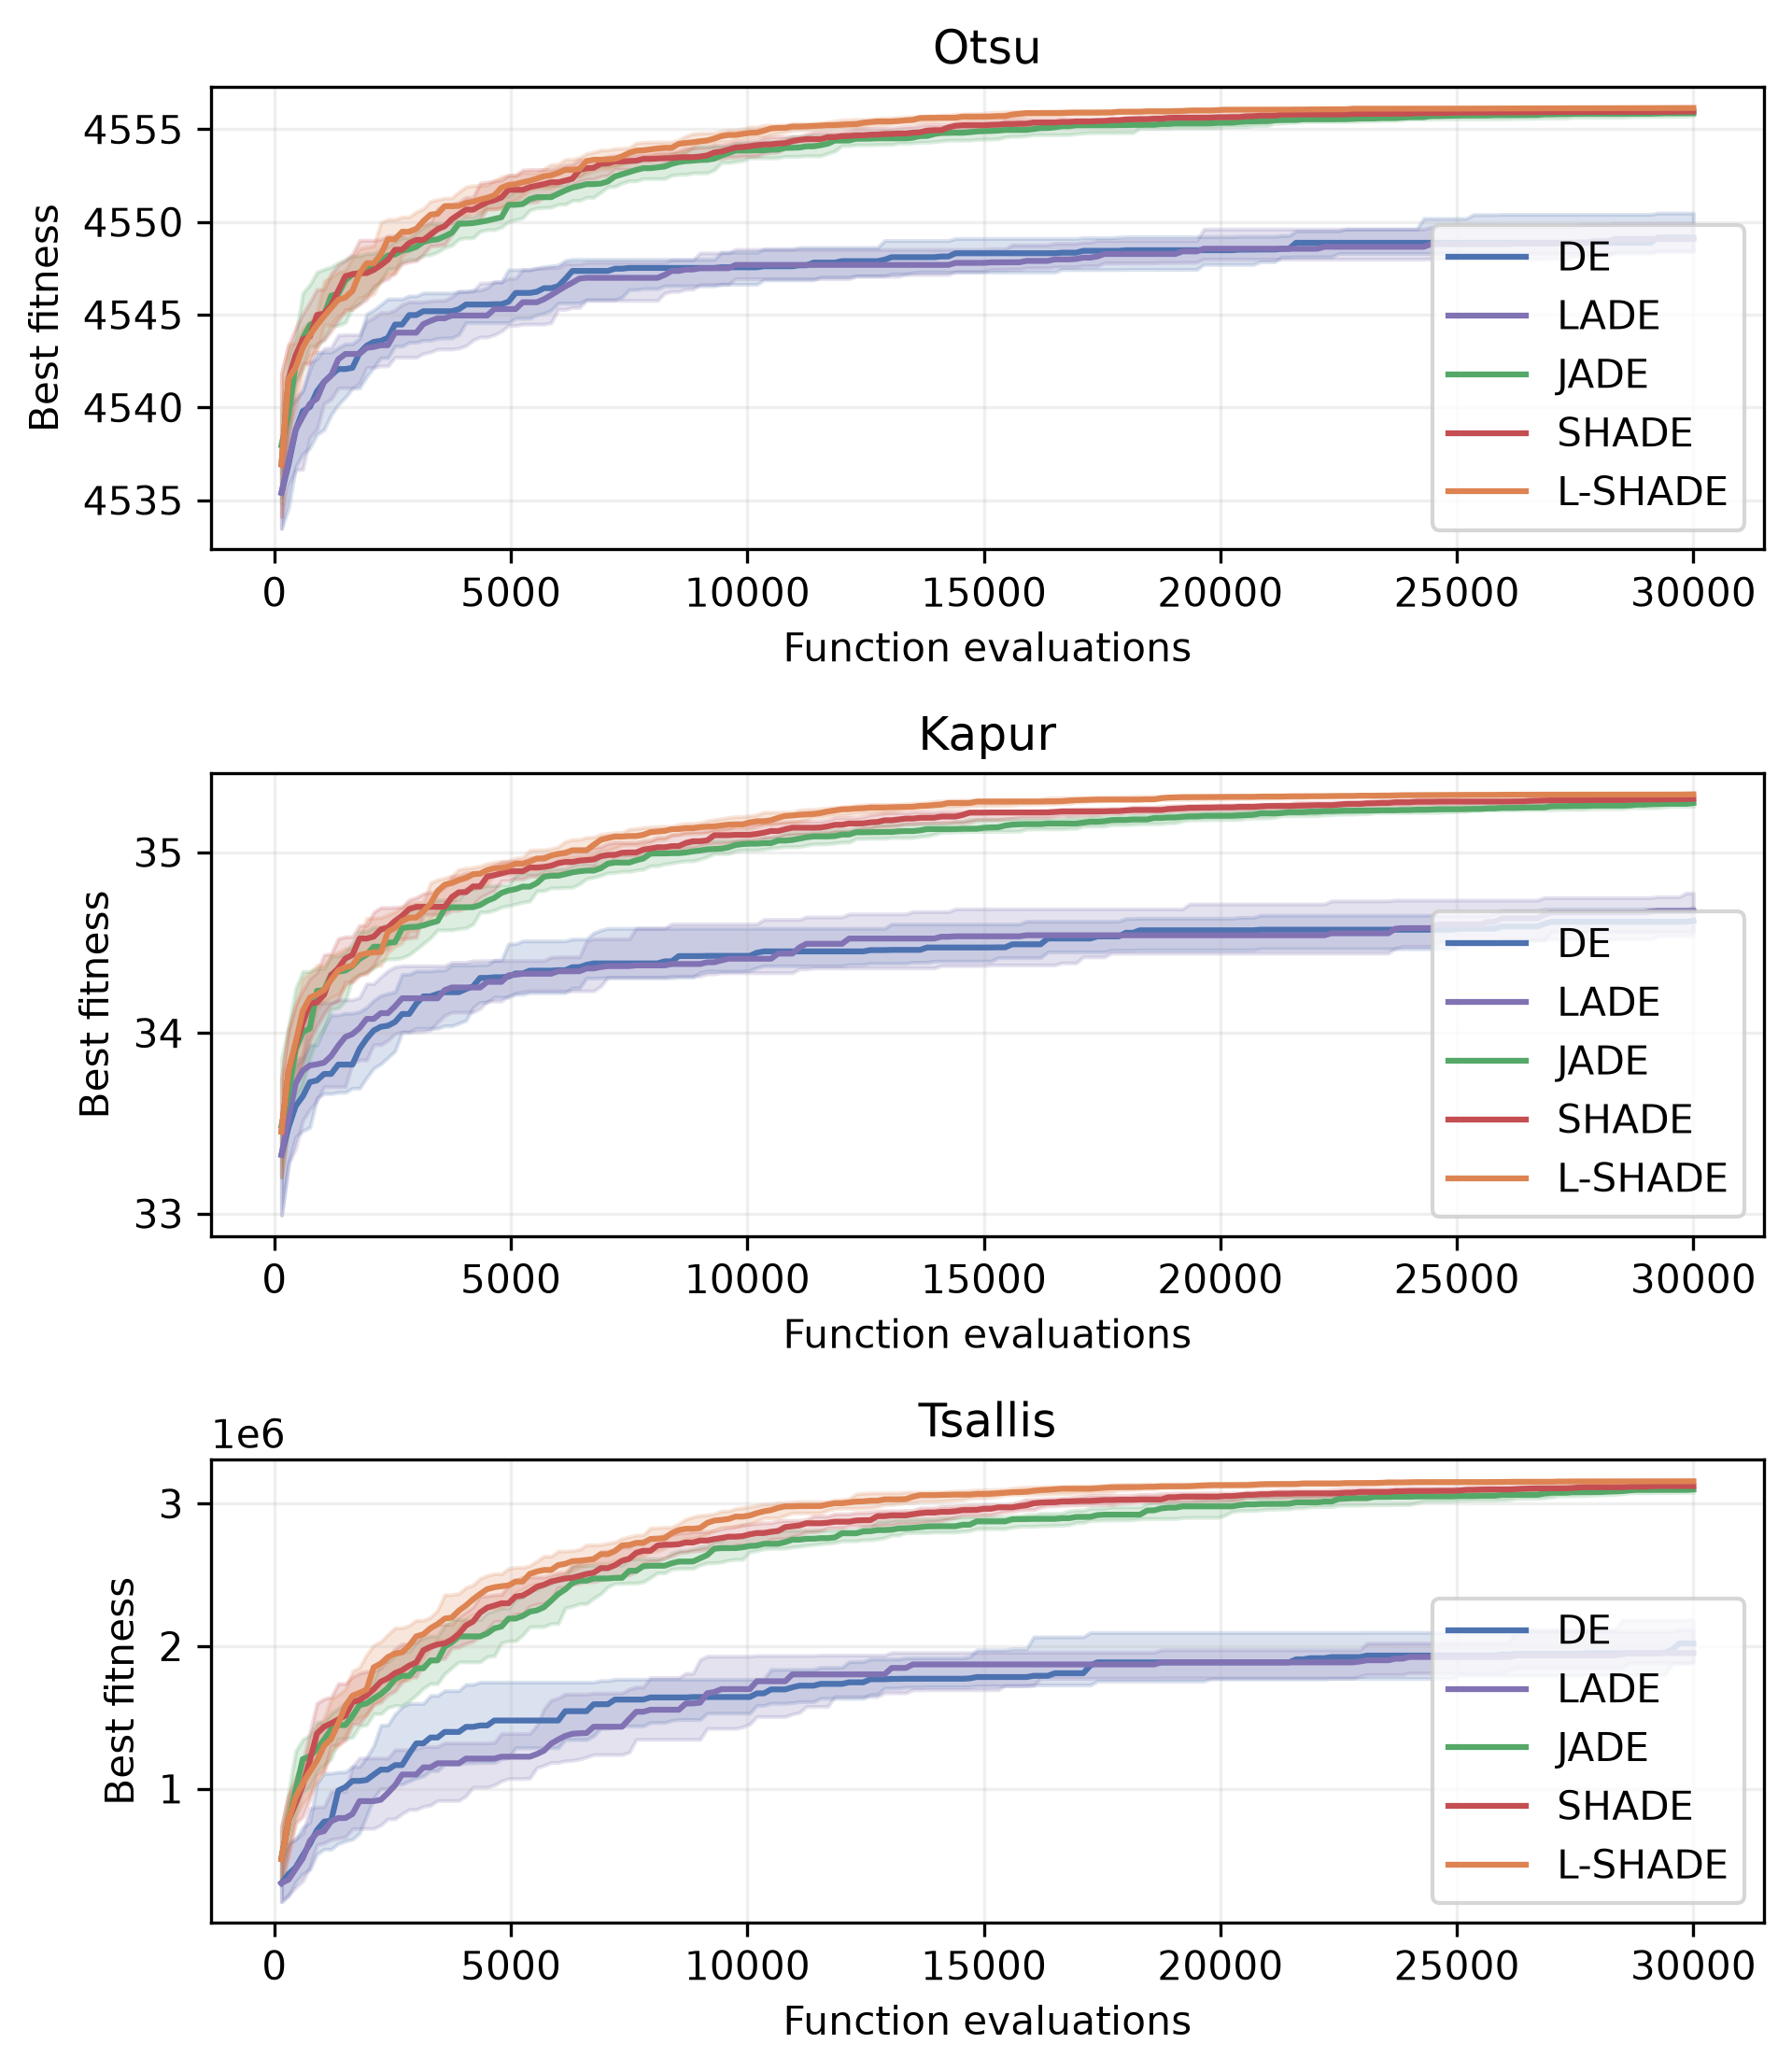
\includegraphics[width=\textwidth]{exp1_convergence.png}

\caption{Best-so-far fitness for img1 at $K=12$. Lines show the median over 30 runs and shaded bands show the interquartile range. Each panel uses its own objective scale; fitness values are not comparable across objectives.}

\label{fig:bsd_convergence}

\end{figure}

Figure~\ref{fig:bsd_convergence} compares convergence under an equal evaluation budget. Best-so-far fitness is retained independently of the current population in LADE, so its curves remain nondecreasing despite acceptance of some worse trials. These curves describe one illustrative image and do not alone establish a dataset-wide convergence advantage.

\subsection{Visual Segmentation Results}

\begin{figure}[htbp]

\centering

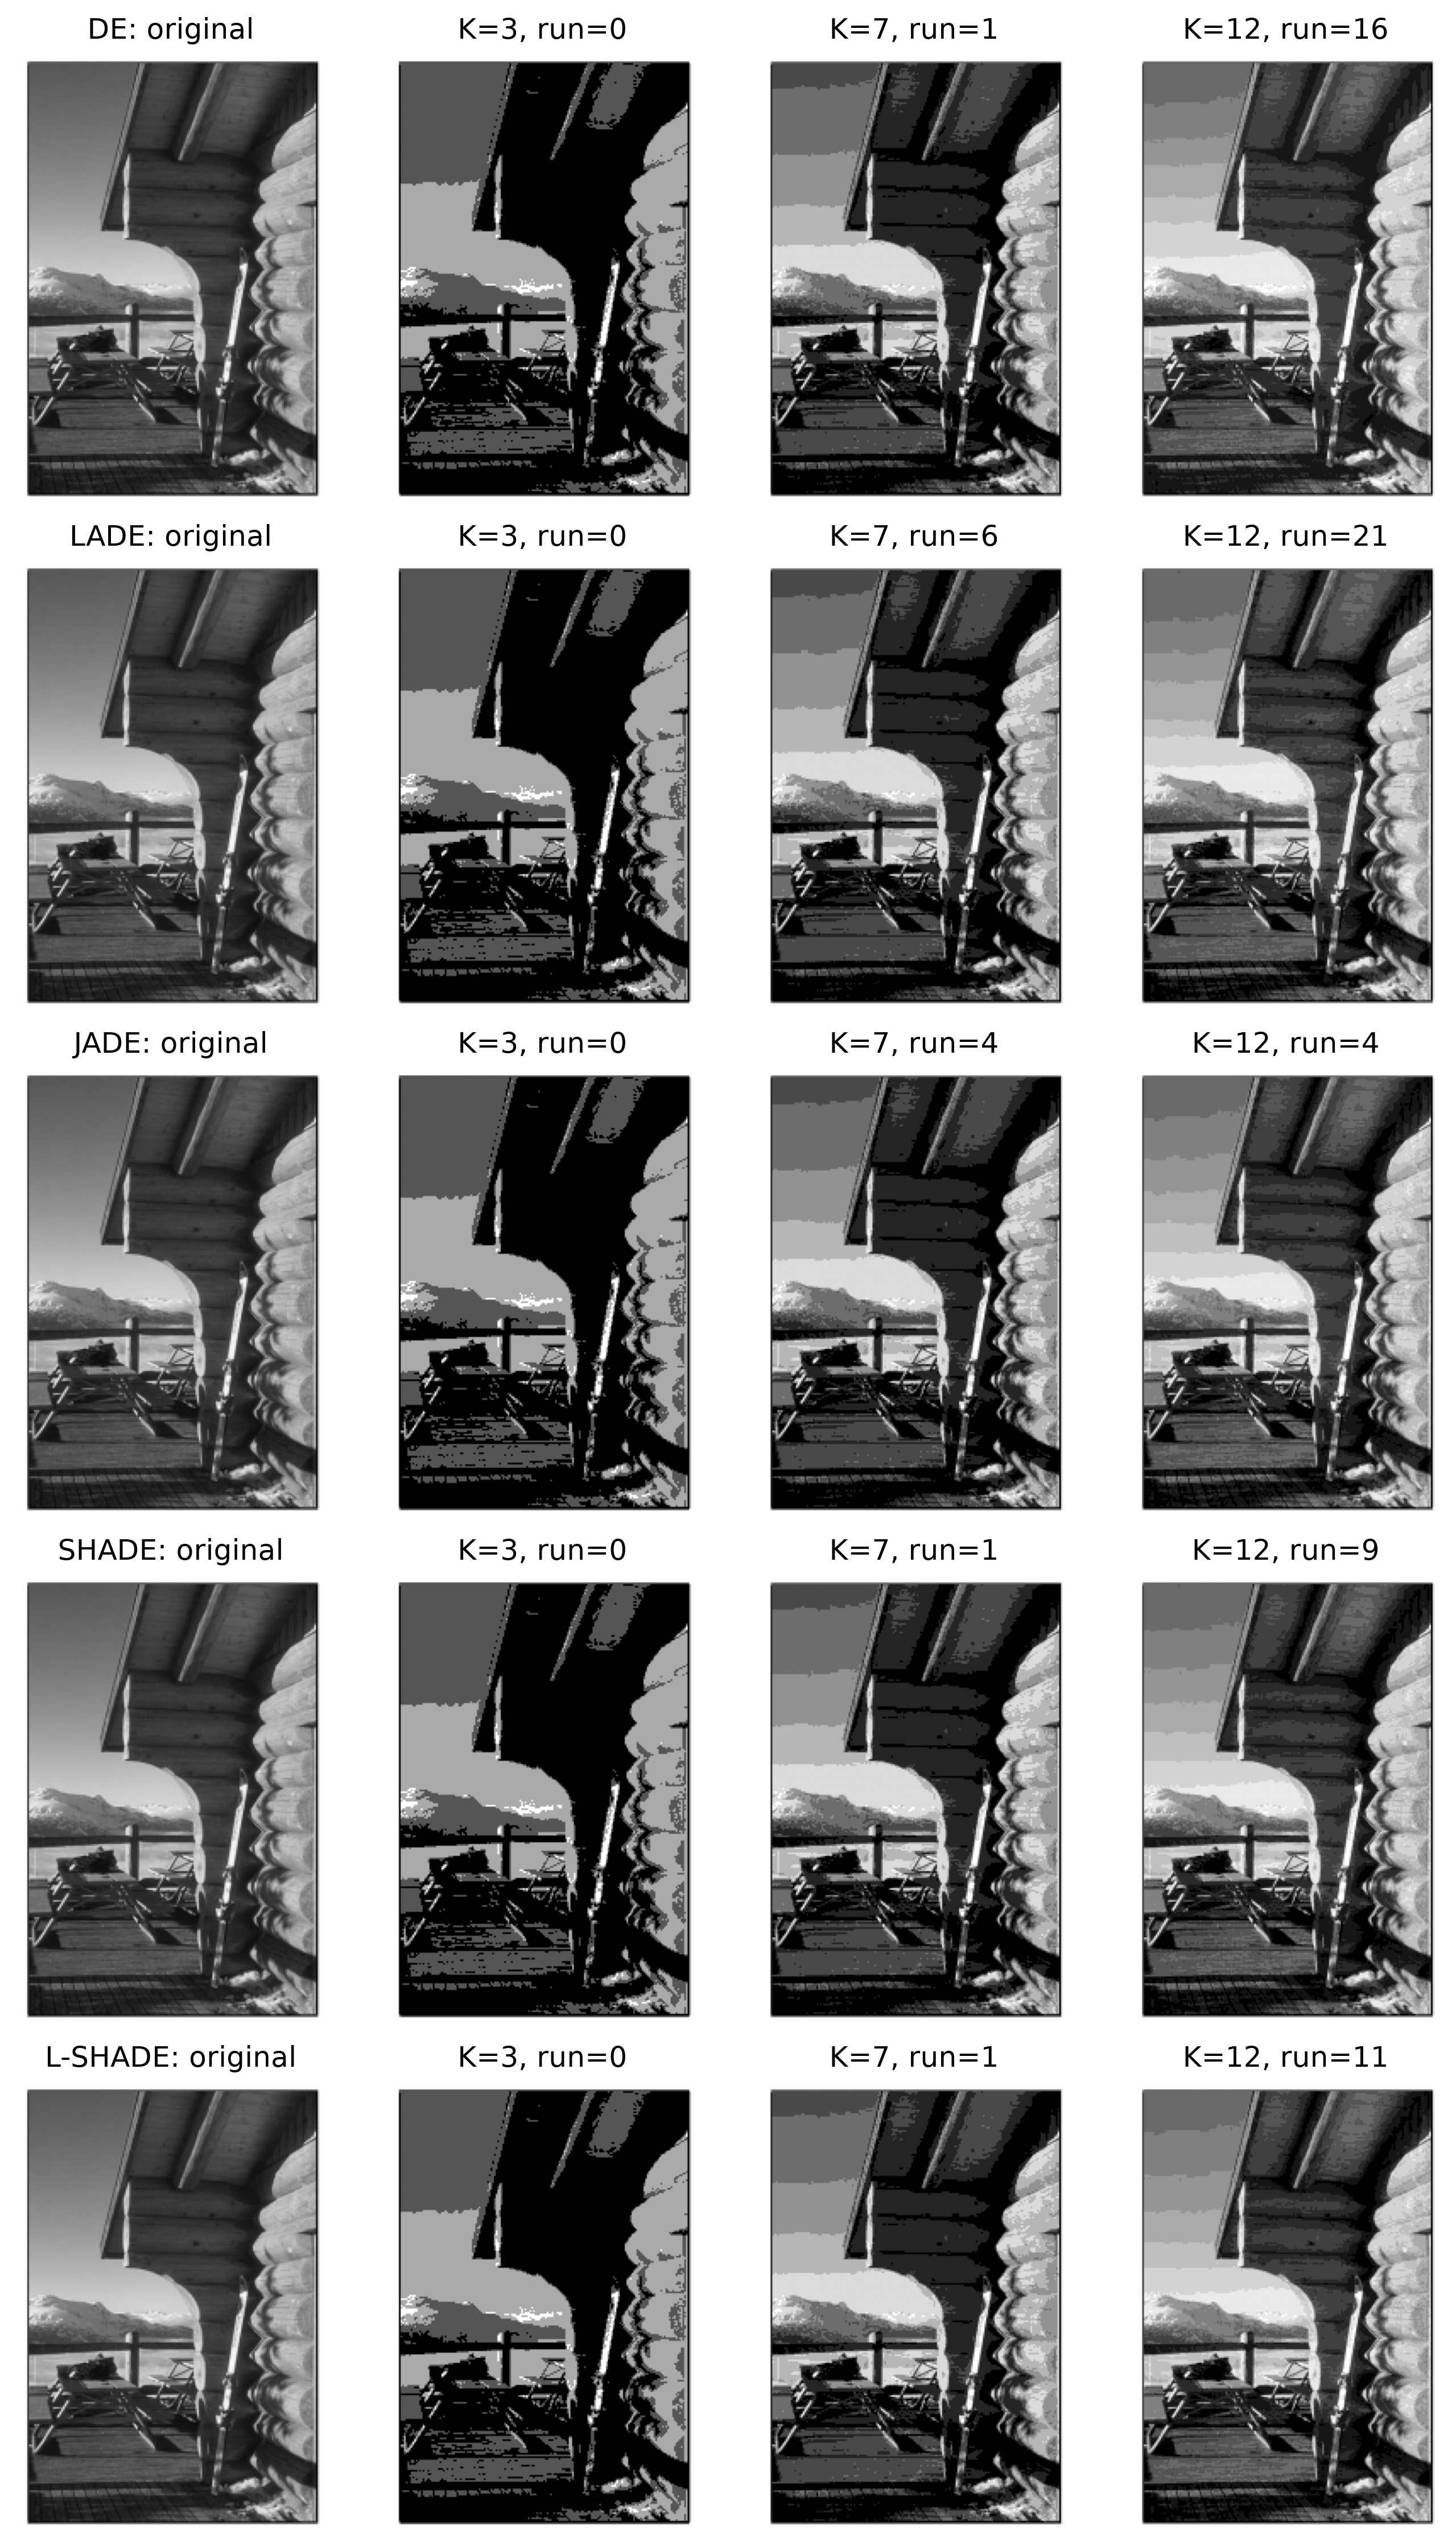
\includegraphics[width=0.9\textwidth]{exp1_segmentation_otsu.png}

\caption{Original and segmented img1 under Otsu at $K=3,7,12$. Rows show DE, LADE, JADE, SHADE and L-SHADE, respectively. Each solution is selected by fitness closest to the median of its 30 runs (ties use the lowest run index). Class intensities are spread evenly for display; PSNR and SSIM are computed using class means instead.}

\label{fig:bsd-segmentation-otsu}

\end{figure}

\begin{figure}[htbp]

\centering

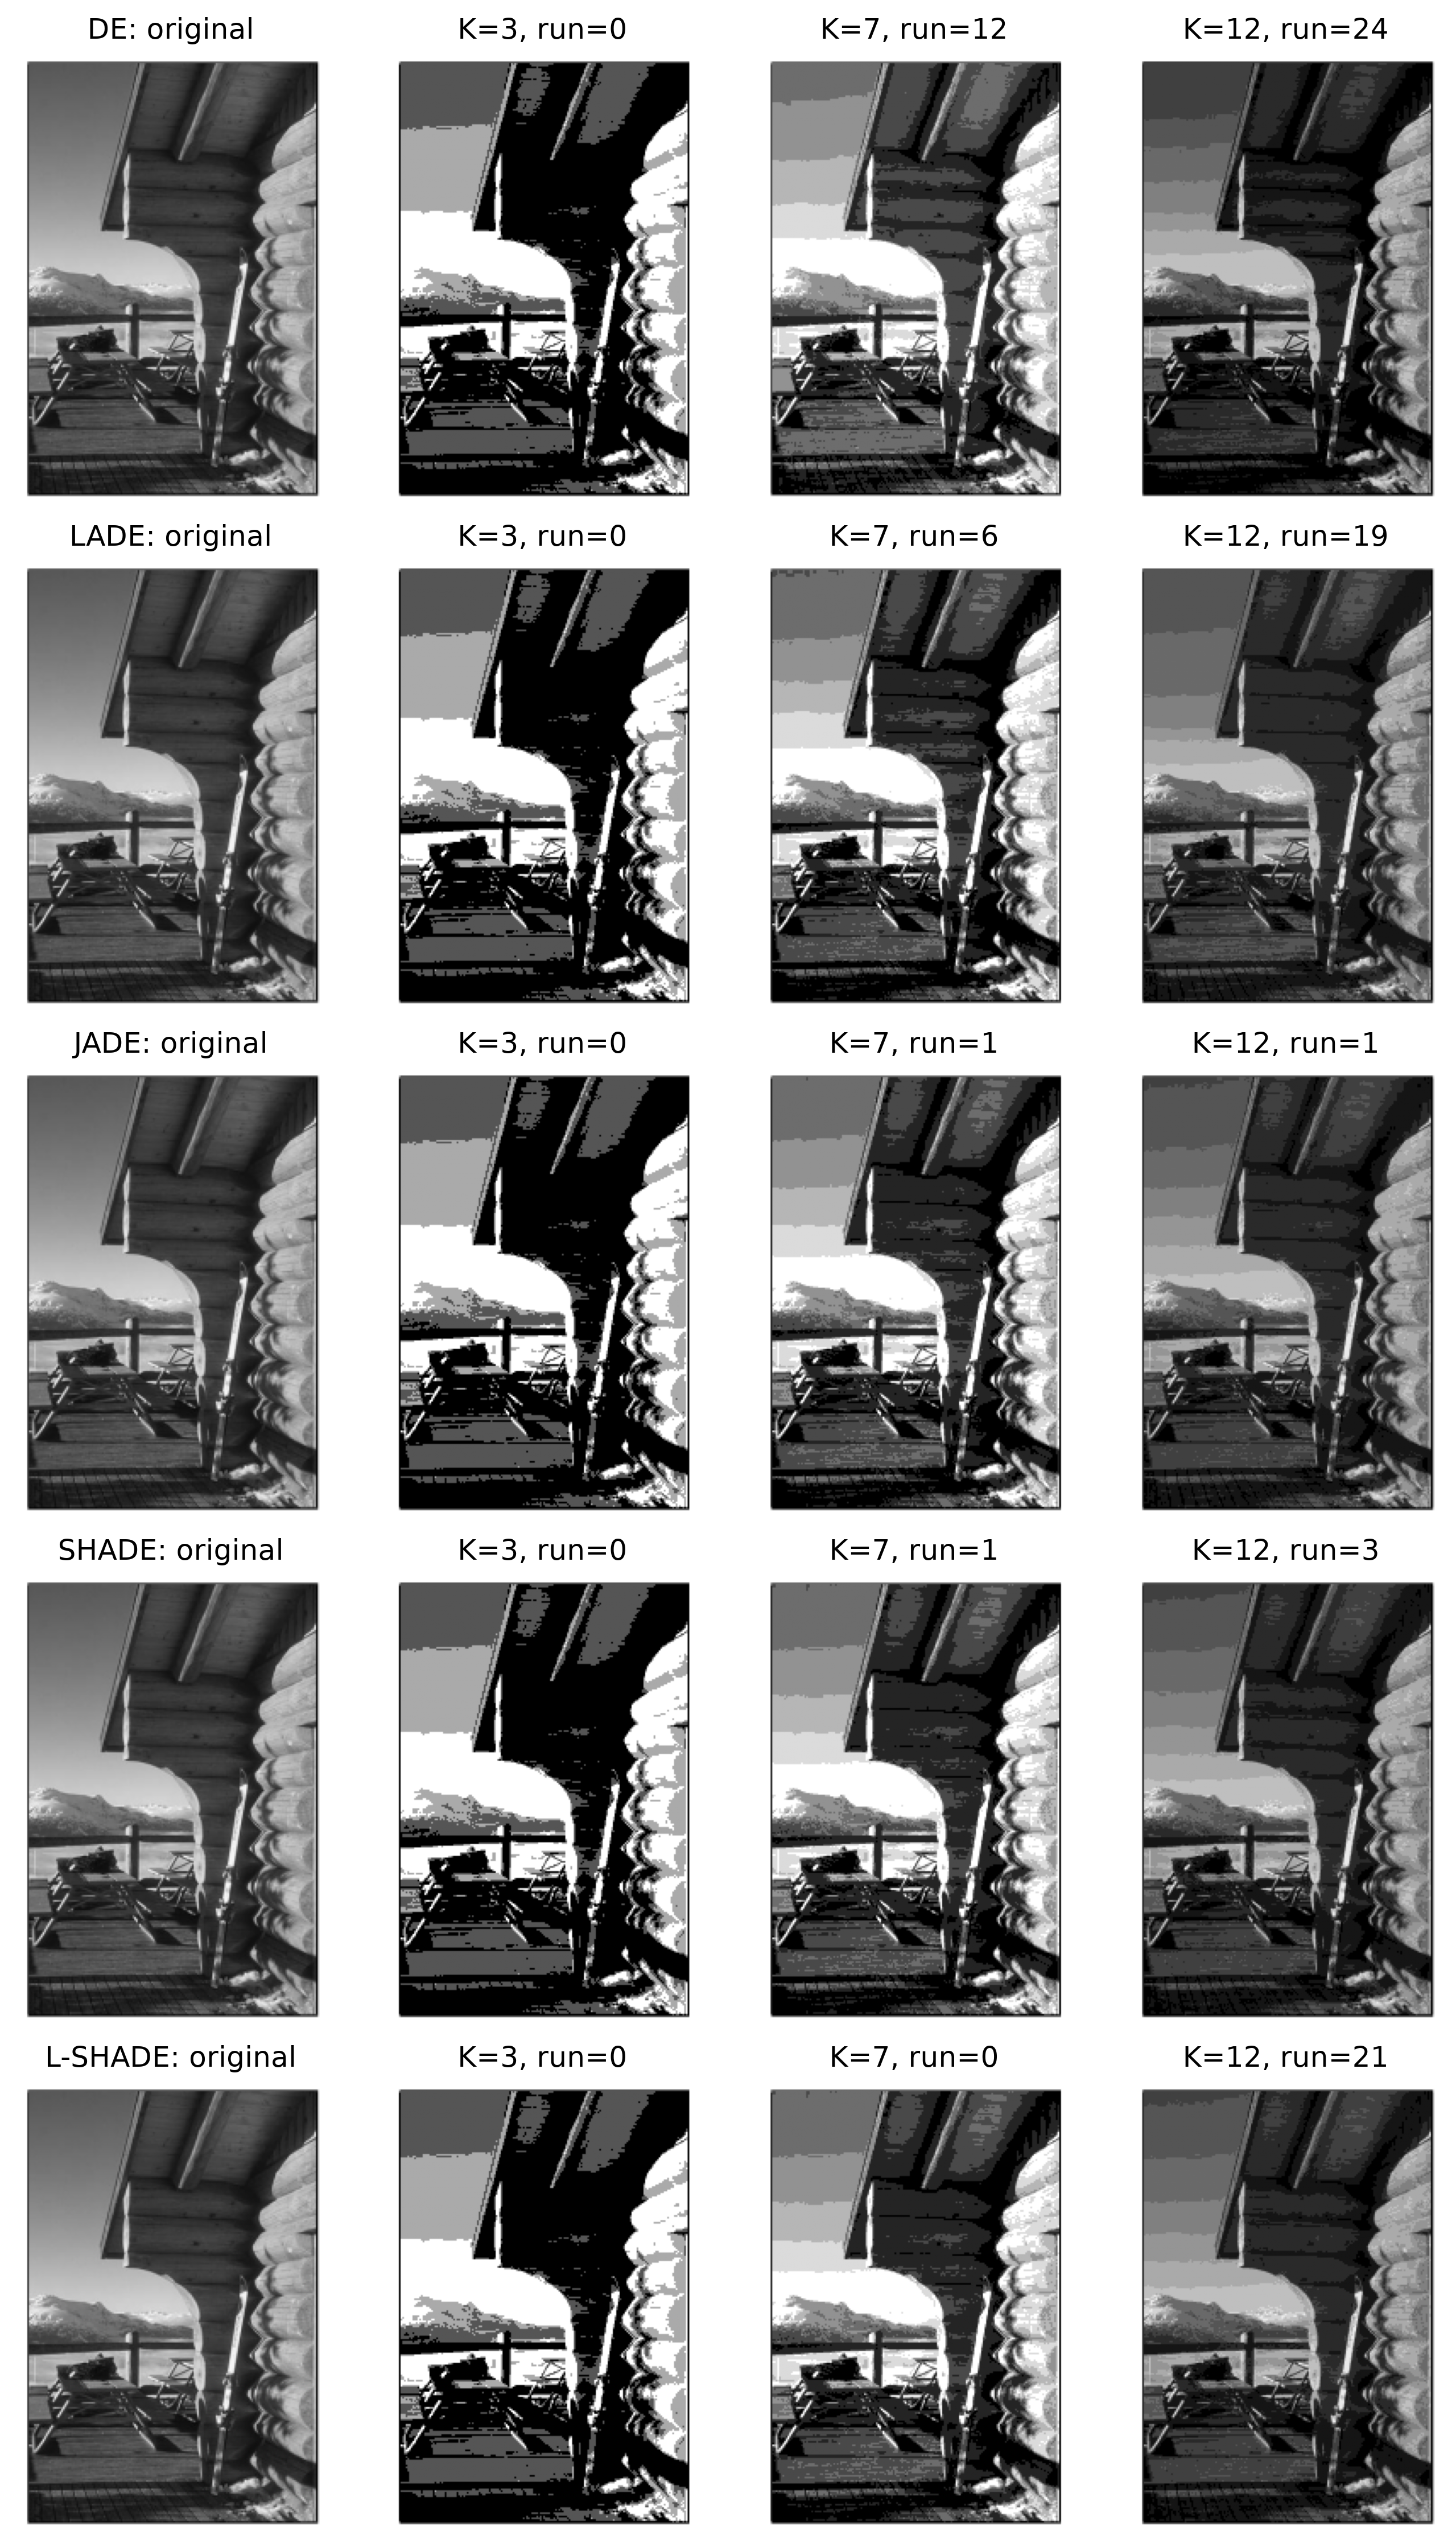
\includegraphics[width=0.9\textwidth]{exp1_segmentation_kapur.png}

\caption{Original and segmented img1 under Kapur at $K=3,7,12$. Rows show DE, LADE, JADE, SHADE and L-SHADE, respectively. Each solution is selected by fitness closest to the median of its 30 runs (ties use the lowest run index). Class intensities are spread evenly for display; PSNR and SSIM are computed using class means instead.}

\label{fig:bsd-segmentation-kapur}

\end{figure}

\begin{figure}[htbp]

\centering

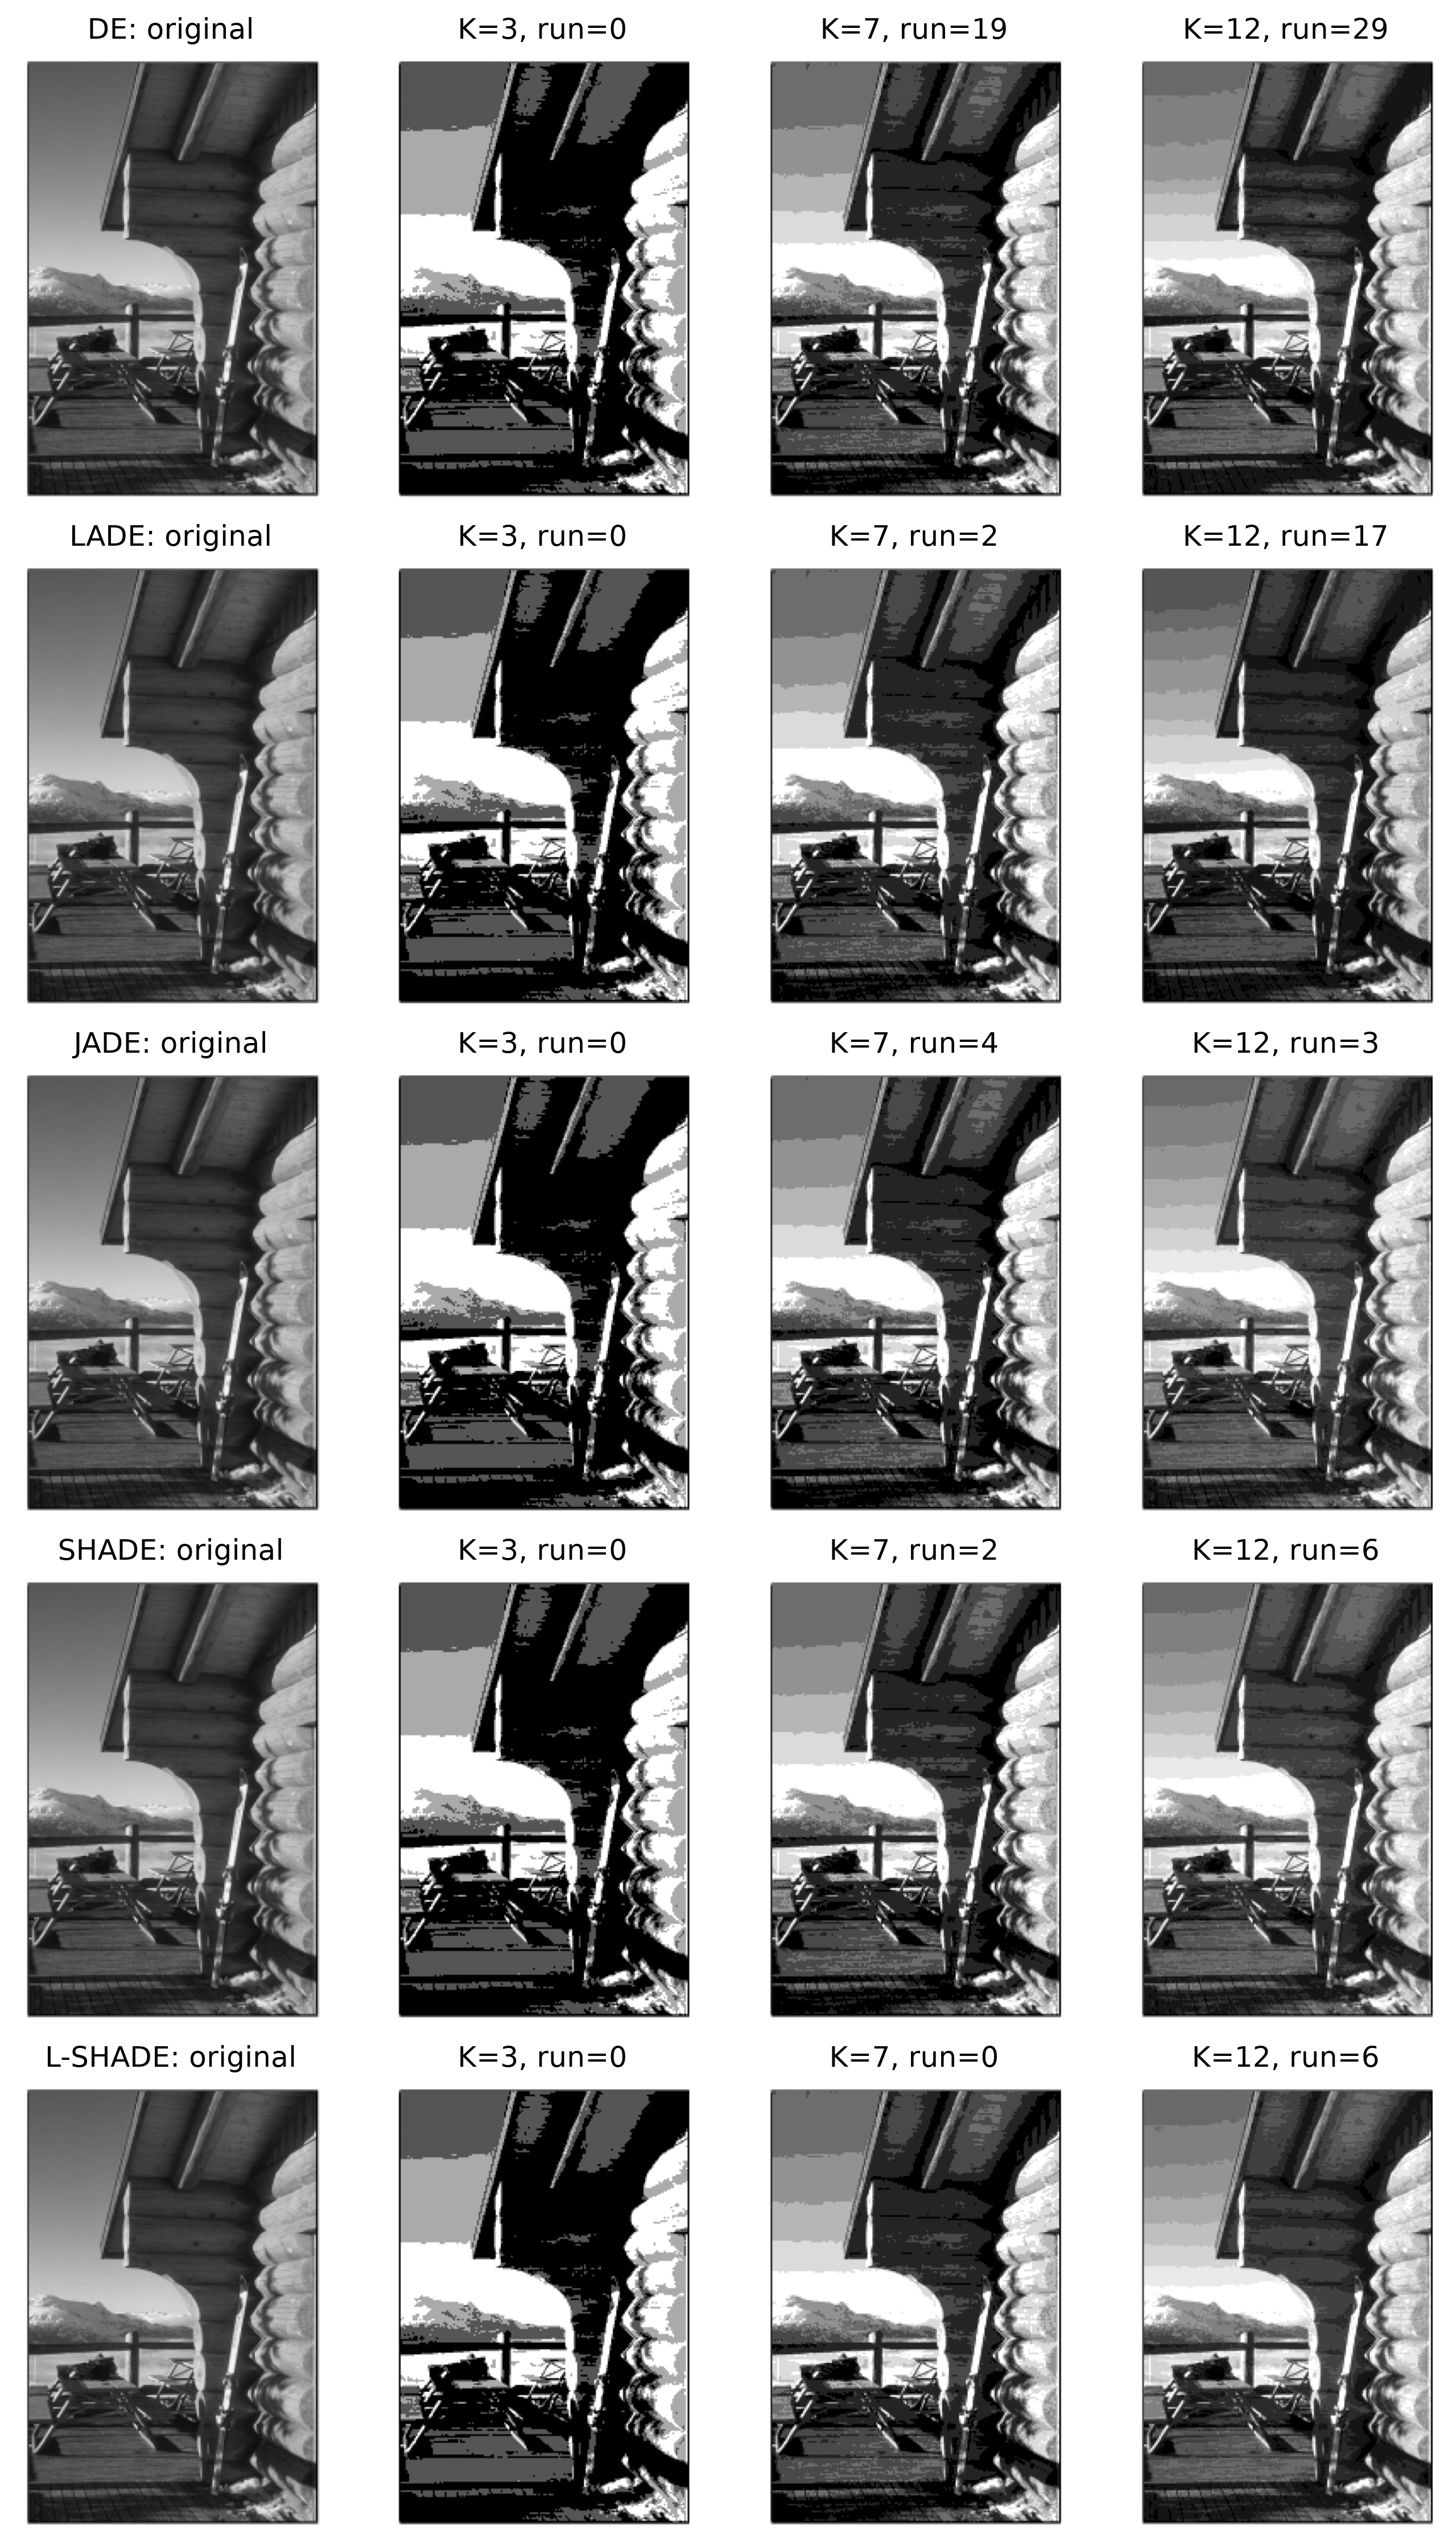
\includegraphics[width=0.9\textwidth]{exp1_segmentation_tsallis.png}

\caption{Original and segmented img1 under Tsallis at $K=3,7,12$. Rows show DE, LADE, JADE, SHADE and L-SHADE, respectively. Each solution is selected by fitness closest to the median of its 30 runs (ties use the lowest run index). Class intensities are spread evenly for display; PSNR and SSIM are computed using class means instead.}

\label{fig:bsd-segmentation-tsallis}

\end{figure}

\clearpage

\subsection{Execution Time}

\begin{figure}[htbp]

\centering

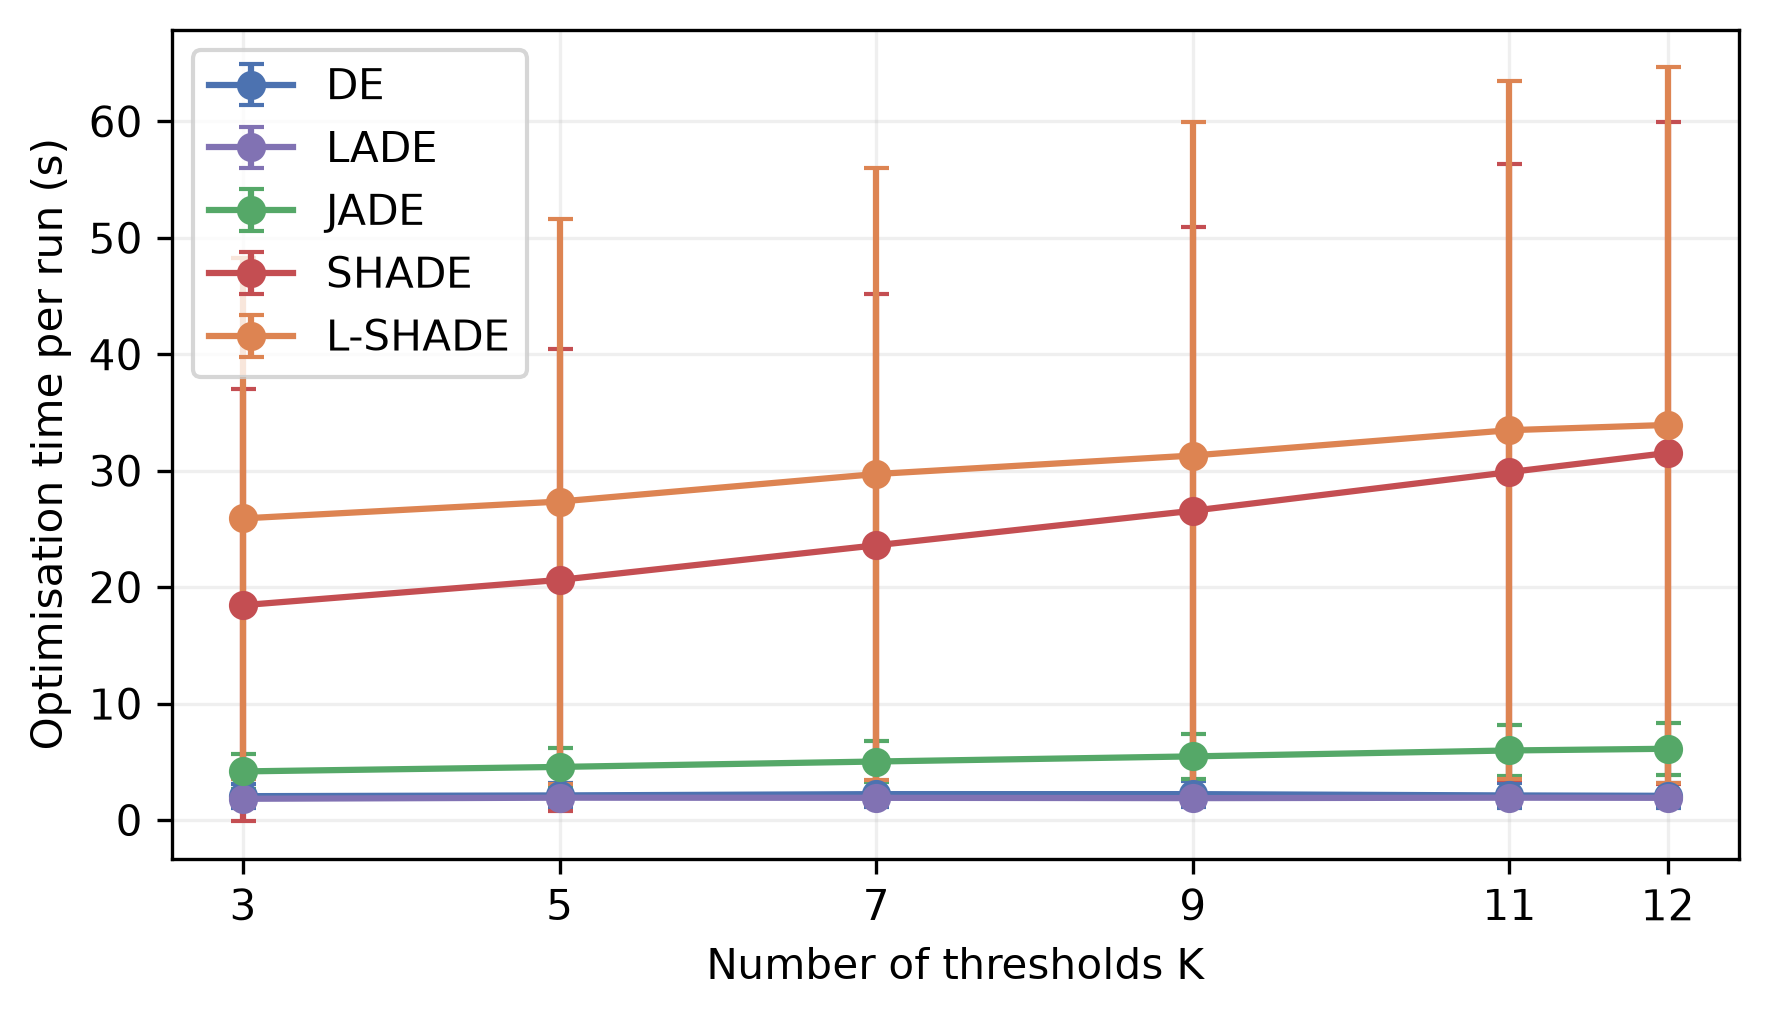
\includegraphics[width=0.8\textwidth]{exp1_runtime.png}

\caption{Mean recorded optimisation time versus $K$. Error bars show sample standard deviation over 900 runs per algorithm and threshold count (10 images, three objectives, 30 runs). DE and LADE were run in separate sweeps, so machine load and worker settings can influence this comparison.}

\label{fig:bsd-runtime}

\end{figure}

Timing covers optimiser execution and objective evaluations using \texttt{time.perf\_counter}; image loading, histogram preparation, exact reference computation, metric calculation and result writing are excluded. The saved results do not record hardware or worker counts, so runtime differences cannot be attributed exclusively to algorithm design.

\subsection{Discussion of Experiment 1}

Across the five algorithms, descriptive differences depend on the objective and threshold count. For the DE--LADE comparison, DE has slightly higher mean Otsu PSNR from $K=7$ through $K=12$, whereas LADE has higher mean Kapur PSNR at $K=5,9,11,12$. At $K=12$, LADE exceeds DE's Kapur PSNR by 0.1906 dB, while DE exceeds LADE's Otsu PSNR by 0.0406 dB. The Otsu results are identical at $K=3$. These small descriptive differences do not demonstrate significant superiority. LADE retains fixed DE control parameters and changes selection through a best-per-history-slot policy; this policy should be considered when interpreting the comparison. The experiment supports the expected improvement in reconstruction with more thresholds and shows that objective choice can have a stronger descriptive effect than switching optimisers. Claims of algorithmic superiority require the paired statistical analysis.

\section{Experiment 2: CHAOS MRI Images}

\label{sec:experiment2}

\subsection{Experimental Objective}

Results for DE, LADE, JADE, SHADE, L-SHADE on 15 CHAOS MRI images, using Otsu, Kapur and Tsallis ($q=0.8$), with $K\in\{3,5,7,9,11,12\}$. Each image--objective--threshold combination contains 30 runs with 30,000 function evaluations per run.

\subsection{Domain-Specific Evaluation}

In accordance with the revised Experiment~2 specification, segmentation
quality on CHAOS is evaluated without ground truth using class separability
$\eta=\sigma_B^2/\sigma_T^2$. This measures how strongly the selected
thresholds separate intensity classes relative to the image's total variance;
higher values indicate more distinct classes.

\subsection{Reconstruction Metrics}

Tables report pooled means and sample standard deviations across images and runs. Dashes indicate unavailable results.

\begin{table}[htbp]
\centering
\small
\caption{PSNR (dB) on CHAOS MRI using Otsu: pooled mean $\pm$ sample standard deviation across 450 observations per entry (15 slices, 30 runs each). Dashes indicate unavailable results.}
\label{tab:chaos-otsu-psnr}
\resizebox{\textwidth}{!}{%
\begin{tabular}{lcccccc}
\toprule
Algorithm & $K=3$ & $K=5$ & $K=7$ & $K=9$ & $K=11$ & $K=12$ \\
\midrule
DE & $27.8831 \pm 0.8927$ & $31.4138 \pm 0.8965$ & $33.8331 \pm 0.9564$ & $35.3458 \pm 0.9609$ & $36.5615 \pm 0.9729$ & $37.1370 \pm 0.9576$ \\
JADE & $27.8831 \pm 0.8927$ & $31.4137 \pm 0.8965$ & $33.9063 \pm 0.9497$ & $35.8694 \pm 0.9423$ & $37.4339 \pm 0.9438$ & $38.1270 \pm 0.9569$ \\
SHADE & $27.8831 \pm 0.8927$ & $31.4138 \pm 0.8965$ & $33.9082 \pm 0.9499$ & $35.8772 \pm 0.9426$ & $37.4524 \pm 0.9433$ & $38.1542 \pm 0.9541$ \\
L-SHADE & $27.8831 \pm 0.8927$ & $31.4138 \pm 0.8965$ & $33.9102 \pm 0.9495$ & $35.8866 \pm 0.9426$ & $37.4741 \pm 0.9422$ & $38.1879 \pm 0.9562$ \\
LADE & $27.8831 \pm 0.8927$ & $31.4138 \pm 0.8965$ & $33.7570 \pm 0.9526$ & $35.2925 \pm 0.9638$ & $36.5373 \pm 0.9430$ & $37.1047 \pm 0.9660$ \\
\bottomrule
\end{tabular}%
}
\end{table}

\begin{table}[htbp]
\centering
\small
\caption{SSIM on CHAOS MRI using Otsu: pooled mean $\pm$ sample standard deviation across 450 observations per entry (15 slices, 30 runs each). Dashes indicate unavailable results.}
\label{tab:chaos-otsu-ssim}
\resizebox{\textwidth}{!}{%
\begin{tabular}{lcccccc}
\toprule
Algorithm & $K=3$ & $K=5$ & $K=7$ & $K=9$ & $K=11$ & $K=12$ \\
\midrule
DE & $0.8664 \pm 0.0411$ & $0.9242 \pm 0.0220$ & $0.9495 \pm 0.0146$ & $0.9612 \pm 0.0120$ & $0.9691 \pm 0.0097$ & $0.9721 \pm 0.0090$ \\
JADE & $0.8664 \pm 0.0411$ & $0.9240 \pm 0.0219$ & $0.9499 \pm 0.0144$ & $0.9643 \pm 0.0109$ & $0.9730 \pm 0.0085$ & $0.9763 \pm 0.0076$ \\
SHADE & $0.8664 \pm 0.0411$ & $0.9240 \pm 0.0219$ & $0.9499 \pm 0.0144$ & $0.9643 \pm 0.0109$ & $0.9731 \pm 0.0085$ & $0.9764 \pm 0.0076$ \\
L-SHADE & $0.8664 \pm 0.0411$ & $0.9240 \pm 0.0219$ & $0.9500 \pm 0.0143$ & $0.9644 \pm 0.0109$ & $0.9732 \pm 0.0084$ & $0.9766 \pm 0.0076$ \\
LADE & $0.8664 \pm 0.0411$ & $0.9243 \pm 0.0220$ & $0.9487 \pm 0.0150$ & $0.9607 \pm 0.0122$ & $0.9688 \pm 0.0098$ & $0.9718 \pm 0.0089$ \\
\bottomrule
\end{tabular}%
}
\end{table}

\begin{table}[htbp]
\centering
\small
\caption{Uniformity on CHAOS MRI using Otsu: pooled mean $\pm$ sample standard deviation across 450 observations per entry (15 slices, 30 runs each). Dashes indicate unavailable results.}
\label{tab:chaos-otsu-uniformity}
\resizebox{\textwidth}{!}{%
\begin{tabular}{lcccccc}
\toprule
Algorithm & $K=3$ & $K=5$ & $K=7$ & $K=9$ & $K=11$ & $K=12$ \\
\midrule
DE & $0.9900 \pm 0.0020$ & $0.9926 \pm 0.0015$ & $0.9941 \pm 0.0012$ & $0.9946 \pm 0.0011$ & $0.9950 \pm 0.0010$ & $0.9953 \pm 0.0010$ \\
JADE & $0.9900 \pm 0.0020$ & $0.9926 \pm 0.0015$ & $0.9942 \pm 0.0012$ & $0.9952 \pm 0.0010$ & $0.9959 \pm 0.0008$ & $0.9962 \pm 0.0008$ \\
SHADE & $0.9900 \pm 0.0020$ & $0.9926 \pm 0.0015$ & $0.9942 \pm 0.0012$ & $0.9952 \pm 0.0010$ & $0.9960 \pm 0.0008$ & $0.9962 \pm 0.0008$ \\
L-SHADE & $0.9900 \pm 0.0020$ & $0.9926 \pm 0.0015$ & $0.9942 \pm 0.0012$ & $0.9953 \pm 0.0010$ & $0.9960 \pm 0.0008$ & $0.9963 \pm 0.0008$ \\
LADE & $0.9900 \pm 0.0020$ & $0.9926 \pm 0.0015$ & $0.9940 \pm 0.0012$ & $0.9946 \pm 0.0011$ & $0.9950 \pm 0.0010$ & $0.9952 \pm 0.0010$ \\
\bottomrule
\end{tabular}%
}
\end{table}

\begin{table}[htbp]
\centering
\small
\caption{Class separability on CHAOS MRI using Otsu: pooled mean $\pm$ sample standard deviation across 450 observations per entry (15 slices, 30 runs each). Dashes indicate unavailable results.}
\label{tab:chaos-otsu-class_separability}
\resizebox{\textwidth}{!}{%
\begin{tabular}{lcccccc}
\toprule
Algorithm & $K=3$ & $K=5$ & $K=7$ & $K=9$ & $K=11$ & $K=12$ \\
\midrule
DE & $0.9760 \pm 0.0076$ & $0.9894 \pm 0.0030$ & $0.9940 \pm 0.0016$ & $0.9957 \pm 0.0011$ & $0.9968 \pm 0.0008$ & $0.9972 \pm 0.0007$ \\
JADE & $0.9760 \pm 0.0076$ & $0.9894 \pm 0.0030$ & $0.9941 \pm 0.0015$ & $0.9962 \pm 0.0010$ & $0.9974 \pm 0.0006$ & $0.9978 \pm 0.0006$ \\
SHADE & $0.9760 \pm 0.0076$ & $0.9894 \pm 0.0030$ & $0.9941 \pm 0.0015$ & $0.9962 \pm 0.0010$ & $0.9974 \pm 0.0006$ & $0.9978 \pm 0.0006$ \\
L-SHADE & $0.9760 \pm 0.0076$ & $0.9894 \pm 0.0030$ & $0.9941 \pm 0.0015$ & $0.9962 \pm 0.0010$ & $0.9974 \pm 0.0006$ & $0.9978 \pm 0.0005$ \\
LADE & $0.9760 \pm 0.0076$ & $0.9894 \pm 0.0030$ & $0.9939 \pm 0.0016$ & $0.9957 \pm 0.0011$ & $0.9968 \pm 0.0008$ & $0.9972 \pm 0.0007$ \\
\bottomrule
\end{tabular}%
}
\end{table}

\begin{table}[htbp]
\centering
\small
\caption{PSNR (dB) on CHAOS MRI using Kapur: pooled mean $\pm$ sample standard deviation across 450 observations per entry (15 slices, 30 runs each). Dashes indicate unavailable results.}
\label{tab:chaos-kapur-psnr}
\resizebox{\textwidth}{!}{%
\begin{tabular}{lcccccc}
\toprule
Algorithm & $K=3$ & $K=5$ & $K=7$ & $K=9$ & $K=11$ & $K=12$ \\
\midrule
DE & $23.9217 \pm 3.2645$ & $29.5546 \pm 1.0739$ & $32.5833 \pm 0.8853$ & $34.2965 \pm 0.9654$ & $35.5513 \pm 1.0270$ & $36.1433 \pm 0.9929$ \\
JADE & $23.9215 \pm 3.2645$ & $29.5506 \pm 1.0778$ & $32.5796 \pm 0.8782$ & $34.6381 \pm 0.9239$ & $36.3703 \pm 0.7912$ & $37.0197 \pm 0.7930$ \\
SHADE & $23.9217 \pm 3.2646$ & $29.5508 \pm 1.0782$ & $32.5807 \pm 0.8757$ & $34.6458 \pm 0.9151$ & $36.3760 \pm 0.7727$ & $37.0522 \pm 0.7896$ \\
L-SHADE & $23.9217 \pm 3.2646$ & $29.5506 \pm 1.0778$ & $32.6031 \pm 0.8709$ & $34.6541 \pm 0.9234$ & $36.3609 \pm 0.7823$ & $37.0286 \pm 0.7541$ \\
LADE & $23.9227 \pm 3.2664$ & $29.5522 \pm 1.0768$ & $32.5398 \pm 0.8799$ & $34.2192 \pm 0.9770$ & $35.5391 \pm 0.9809$ & $36.1674 \pm 1.0023$ \\
\bottomrule
\end{tabular}%
}
\end{table}

\begin{table}[htbp]
\centering
\small
\caption{SSIM on CHAOS MRI using Kapur: pooled mean $\pm$ sample standard deviation across 450 observations per entry (15 slices, 30 runs each). Dashes indicate unavailable results.}
\label{tab:chaos-kapur-ssim}
\resizebox{\textwidth}{!}{%
\begin{tabular}{lcccccc}
\toprule
Algorithm & $K=3$ & $K=5$ & $K=7$ & $K=9$ & $K=11$ & $K=12$ \\
\midrule
DE & $0.6508 \pm 0.2917$ & $0.9107 \pm 0.0267$ & $0.9398 \pm 0.0166$ & $0.9537 \pm 0.0136$ & $0.9625 \pm 0.0118$ & $0.9662 \pm 0.0106$ \\
JADE & $0.6508 \pm 0.2917$ & $0.9106 \pm 0.0268$ & $0.9396 \pm 0.0163$ & $0.9551 \pm 0.0133$ & $0.9661 \pm 0.0105$ & $0.9694 \pm 0.0098$ \\
SHADE & $0.6508 \pm 0.2917$ & $0.9106 \pm 0.0268$ & $0.9397 \pm 0.0162$ & $0.9551 \pm 0.0133$ & $0.9661 \pm 0.0103$ & $0.9696 \pm 0.0097$ \\
L-SHADE & $0.6508 \pm 0.2917$ & $0.9106 \pm 0.0268$ & $0.9397 \pm 0.0161$ & $0.9551 \pm 0.0133$ & $0.9660 \pm 0.0104$ & $0.9694 \pm 0.0097$ \\
LADE & $0.6509 \pm 0.2916$ & $0.9107 \pm 0.0268$ & $0.9395 \pm 0.0164$ & $0.9532 \pm 0.0139$ & $0.9625 \pm 0.0117$ & $0.9662 \pm 0.0108$ \\
\bottomrule
\end{tabular}%
}
\end{table}

\begin{table}[htbp]
\centering
\small
\caption{Uniformity on CHAOS MRI using Kapur: pooled mean $\pm$ sample standard deviation across 450 observations per entry (15 slices, 30 runs each). Dashes indicate unavailable results.}
\label{tab:chaos-kapur-uniformity}
\resizebox{\textwidth}{!}{%
\begin{tabular}{lcccccc}
\toprule
Algorithm & $K=3$ & $K=5$ & $K=7$ & $K=9$ & $K=11$ & $K=12$ \\
\midrule
DE & $0.9654 \pm 0.0376$ & $0.9886 \pm 0.0031$ & $0.9921 \pm 0.0016$ & $0.9931 \pm 0.0015$ & $0.9937 \pm 0.0015$ & $0.9940 \pm 0.0014$ \\
JADE & $0.9654 \pm 0.0376$ & $0.9885 \pm 0.0031$ & $0.9921 \pm 0.0015$ & $0.9937 \pm 0.0013$ & $0.9948 \pm 0.0009$ & $0.9952 \pm 0.0009$ \\
SHADE & $0.9654 \pm 0.0376$ & $0.9885 \pm 0.0031$ & $0.9921 \pm 0.0015$ & $0.9937 \pm 0.0013$ & $0.9949 \pm 0.0009$ & $0.9952 \pm 0.0009$ \\
L-SHADE & $0.9654 \pm 0.0376$ & $0.9885 \pm 0.0031$ & $0.9922 \pm 0.0015$ & $0.9937 \pm 0.0013$ & $0.9948 \pm 0.0009$ & $0.9952 \pm 0.0008$ \\
LADE & $0.9654 \pm 0.0376$ & $0.9885 \pm 0.0031$ & $0.9920 \pm 0.0016$ & $0.9930 \pm 0.0016$ & $0.9937 \pm 0.0014$ & $0.9940 \pm 0.0014$ \\
\bottomrule
\end{tabular}%
}
\end{table}

\begin{table}[htbp]
\centering
\small
\caption{Class separability on CHAOS MRI using Kapur: pooled mean $\pm$ sample standard deviation across 450 observations per entry (15 slices, 30 runs each). Dashes indicate unavailable results.}
\label{tab:chaos-kapur-class_separability}
\resizebox{\textwidth}{!}{%
\begin{tabular}{lcccccc}
\toprule
Algorithm & $K=3$ & $K=5$ & $K=7$ & $K=9$ & $K=11$ & $K=12$ \\
\midrule
DE & $0.9105 \pm 0.0956$ & $0.9836 \pm 0.0056$ & $0.9919 \pm 0.0024$ & $0.9945 \pm 0.0016$ & $0.9959 \pm 0.0013$ & $0.9964 \pm 0.0012$ \\
JADE & $0.9105 \pm 0.0956$ & $0.9835 \pm 0.0056$ & $0.9919 \pm 0.0023$ & $0.9950 \pm 0.0015$ & $0.9966 \pm 0.0010$ & $0.9971 \pm 0.0009$ \\
SHADE & $0.9105 \pm 0.0956$ & $0.9835 \pm 0.0056$ & $0.9919 \pm 0.0022$ & $0.9950 \pm 0.0015$ & $0.9966 \pm 0.0010$ & $0.9971 \pm 0.0008$ \\
L-SHADE & $0.9105 \pm 0.0956$ & $0.9835 \pm 0.0056$ & $0.9920 \pm 0.0023$ & $0.9950 \pm 0.0015$ & $0.9966 \pm 0.0010$ & $0.9971 \pm 0.0009$ \\
LADE & $0.9104 \pm 0.0959$ & $0.9835 \pm 0.0056$ & $0.9918 \pm 0.0023$ & $0.9944 \pm 0.0018$ & $0.9959 \pm 0.0013$ & $0.9964 \pm 0.0011$ \\
\bottomrule
\end{tabular}%
}
\end{table}

\begin{table}[htbp]
\centering
\small
\caption{PSNR (dB) on CHAOS MRI using Tsallis ($q=0.8$): pooled mean $\pm$ sample standard deviation across 450 observations per entry (15 slices, 30 runs each). Dashes indicate unavailable results.}
\label{tab:chaos-tsallis-psnr}
\resizebox{\textwidth}{!}{%
\begin{tabular}{lcccccc}
\toprule
Algorithm & $K=3$ & $K=5$ & $K=7$ & $K=9$ & $K=11$ & $K=12$ \\
\midrule
DE & $19.2215 \pm 1.6472$ & $21.6107 \pm 1.1139$ & $23.3961 \pm 1.3927$ & $25.6068 \pm 2.0485$ & $30.6101 \pm 3.6384$ & $32.5967 \pm 3.4584$ \\
JADE & $19.2181 \pm 1.6513$ & $21.6330 \pm 1.1308$ & $23.2566 \pm 1.2368$ & $24.9454 \pm 1.4385$ & $28.0967 \pm 2.9150$ & $31.8020 \pm 3.9910$ \\
SHADE & $19.2196 \pm 1.6494$ & $21.6346 \pm 1.1324$ & $23.2030 \pm 1.2253$ & $24.9350 \pm 1.4466$ & $27.9417 \pm 2.9986$ & $31.8170 \pm 3.9610$ \\
L-SHADE & $19.2181 \pm 1.6513$ & $21.6353 \pm 1.1324$ & $23.2081 \pm 1.2007$ & $24.8569 \pm 1.4351$ & $27.8754 \pm 2.9272$ & $31.8367 \pm 3.9782$ \\
LADE & $19.2181 \pm 1.6513$ & $21.6014 \pm 1.1181$ & $23.3535 \pm 1.4040$ & $25.7208 \pm 2.1794$ & $30.5670 \pm 3.6296$ & $32.6407 \pm 3.6075$ \\
\bottomrule
\end{tabular}%
}
\end{table}

\begin{table}[htbp]
\centering
\small
\caption{SSIM on CHAOS MRI using Tsallis ($q=0.8$): pooled mean $\pm$ sample standard deviation across 450 observations per entry (15 slices, 30 runs each). Dashes indicate unavailable results.}
\label{tab:chaos-tsallis-ssim}
\resizebox{\textwidth}{!}{%
\begin{tabular}{lcccccc}
\toprule
Algorithm & $K=3$ & $K=5$ & $K=7$ & $K=9$ & $K=11$ & $K=12$ \\
\midrule
DE & $0.2651 \pm 0.0369$ & $0.3339 \pm 0.0454$ & $0.3942 \pm 0.0607$ & $0.4913 \pm 0.1030$ & $0.7339 \pm 0.1884$ & $0.8163 \pm 0.1675$ \\
JADE & $0.2650 \pm 0.0370$ & $0.3347 \pm 0.0437$ & $0.3883 \pm 0.0609$ & $0.4556 \pm 0.0672$ & $0.6043 \pm 0.1512$ & $0.7612 \pm 0.1839$ \\
SHADE & $0.2650 \pm 0.0370$ & $0.3347 \pm 0.0437$ & $0.3867 \pm 0.0601$ & $0.4551 \pm 0.0678$ & $0.5962 \pm 0.1538$ & $0.7616 \pm 0.1819$ \\
L-SHADE & $0.2650 \pm 0.0370$ & $0.3347 \pm 0.0437$ & $0.3867 \pm 0.0593$ & $0.4517 \pm 0.0660$ & $0.5932 \pm 0.1514$ & $0.7619 \pm 0.1830$ \\
LADE & $0.2650 \pm 0.0370$ & $0.3337 \pm 0.0457$ & $0.3926 \pm 0.0598$ & $0.4968 \pm 0.1153$ & $0.7298 \pm 0.1886$ & $0.8167 \pm 0.1745$ \\
\bottomrule
\end{tabular}%
}
\end{table}

\begin{table}[htbp]
\centering
\small
\caption{Uniformity on CHAOS MRI using Tsallis ($q=0.8$): pooled mean $\pm$ sample standard deviation across 450 observations per entry (15 slices, 30 runs each). Dashes indicate unavailable results.}
\label{tab:chaos-tsallis-uniformity}
\resizebox{\textwidth}{!}{%
\begin{tabular}{lcccccc}
\toprule
Algorithm & $K=3$ & $K=5$ & $K=7$ & $K=9$ & $K=11$ & $K=12$ \\
\midrule
DE & $0.9225 \pm 0.0328$ & $0.9287 \pm 0.0184$ & $0.9326 \pm 0.0219$ & $0.9449 \pm 0.0258$ & $0.9728 \pm 0.0247$ & $0.9813 \pm 0.0185$ \\
JADE & $0.9224 \pm 0.0329$ & $0.9290 \pm 0.0186$ & $0.9311 \pm 0.0196$ & $0.9391 \pm 0.0207$ & $0.9593 \pm 0.0209$ & $0.9768 \pm 0.0183$ \\
SHADE & $0.9225 \pm 0.0329$ & $0.9290 \pm 0.0186$ & $0.9303 \pm 0.0197$ & $0.9389 \pm 0.0207$ & $0.9572 \pm 0.0236$ & $0.9770 \pm 0.0179$ \\
L-SHADE & $0.9224 \pm 0.0329$ & $0.9290 \pm 0.0187$ & $0.9305 \pm 0.0193$ & $0.9379 \pm 0.0208$ & $0.9571 \pm 0.0223$ & $0.9771 \pm 0.0176$ \\
LADE & $0.9224 \pm 0.0329$ & $0.9285 \pm 0.0184$ & $0.9318 \pm 0.0227$ & $0.9458 \pm 0.0258$ & $0.9730 \pm 0.0227$ & $0.9809 \pm 0.0193$ \\
\bottomrule
\end{tabular}%
}
\end{table}

\begin{table}[htbp]
\centering
\small
\caption{Class separability on CHAOS MRI using Tsallis ($q=0.8$): pooled mean $\pm$ sample standard deviation across 450 observations per entry (15 slices, 30 runs each). Dashes indicate unavailable results.}
\label{tab:chaos-tsallis-class_separability}
\resizebox{\textwidth}{!}{%
\begin{tabular}{lcccccc}
\toprule
Algorithm & $K=3$ & $K=5$ & $K=7$ & $K=9$ & $K=11$ & $K=12$ \\
\midrule
DE & $0.8130 \pm 0.0917$ & $0.8968 \pm 0.0393$ & $0.9292 \pm 0.0325$ & $0.9553 \pm 0.0240$ & $0.9804 \pm 0.0202$ & $0.9868 \pm 0.0166$ \\
JADE & $0.8128 \pm 0.0919$ & $0.8981 \pm 0.0340$ & $0.9266 \pm 0.0345$ & $0.9508 \pm 0.0196$ & $0.9719 \pm 0.0164$ & $0.9841 \pm 0.0146$ \\
SHADE & $0.8129 \pm 0.0918$ & $0.8982 \pm 0.0340$ & $0.9258 \pm 0.0346$ & $0.9507 \pm 0.0196$ & $0.9707 \pm 0.0177$ & $0.9843 \pm 0.0147$ \\
L-SHADE & $0.8128 \pm 0.0919$ & $0.8982 \pm 0.0340$ & $0.9259 \pm 0.0345$ & $0.9500 \pm 0.0193$ & $0.9705 \pm 0.0171$ & $0.9842 \pm 0.0149$ \\
LADE & $0.8128 \pm 0.0919$ & $0.8963 \pm 0.0406$ & $0.9286 \pm 0.0324$ & $0.9558 \pm 0.0240$ & $0.9801 \pm 0.0202$ & $0.9864 \pm 0.0170$ \\
\bottomrule
\end{tabular}%
}
\end{table}

\subsection{Visual MRI Segmentation Results}

\begin{figure}[htbp]
\centering
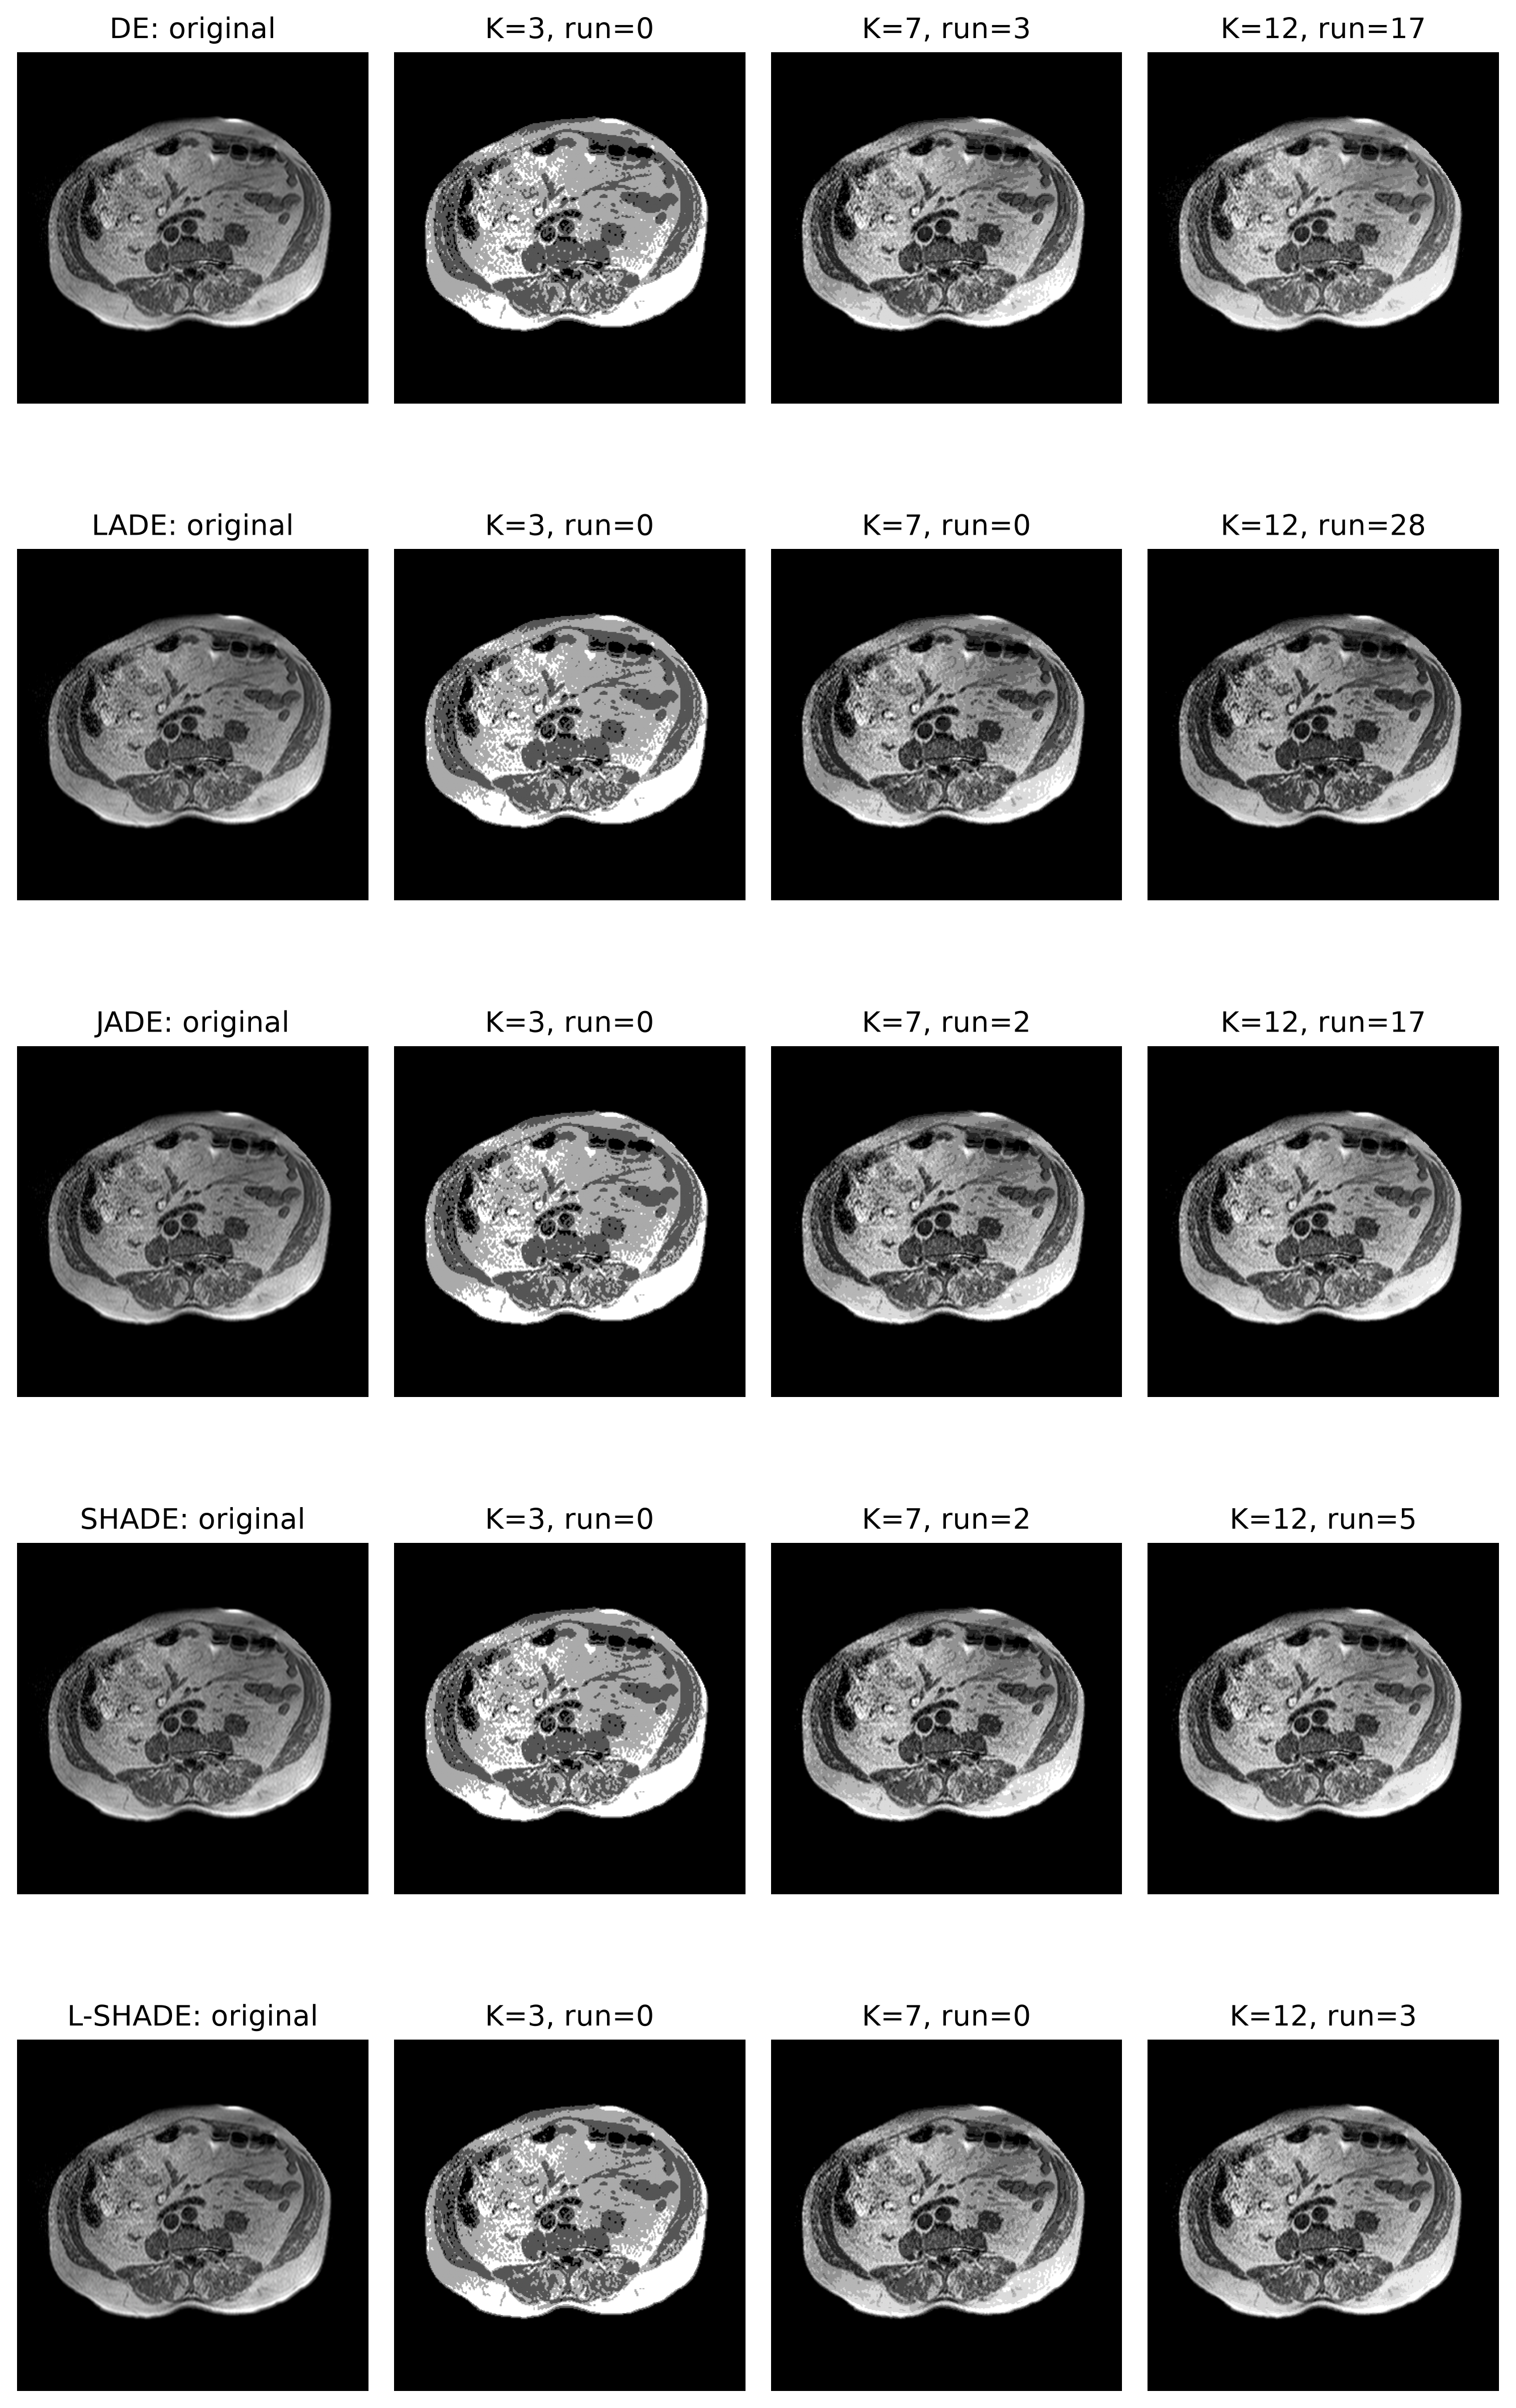
\includegraphics[width=0.9\textwidth]{exp2_segmentation_otsu.png}
\caption{Original and thresholded image IMG-0003-00010 using Otsu at $K=3,7,12$. Rows: DE, LADE, JADE, SHADE, L-SHADE. Solutions are selected by final fitness closest to the median, with ties resolved by the lowest run index. The displayed run number identifies an independent repetition.}
\label{fig:chaos-otsu}
\end{figure}

\begin{figure}[htbp]
\centering
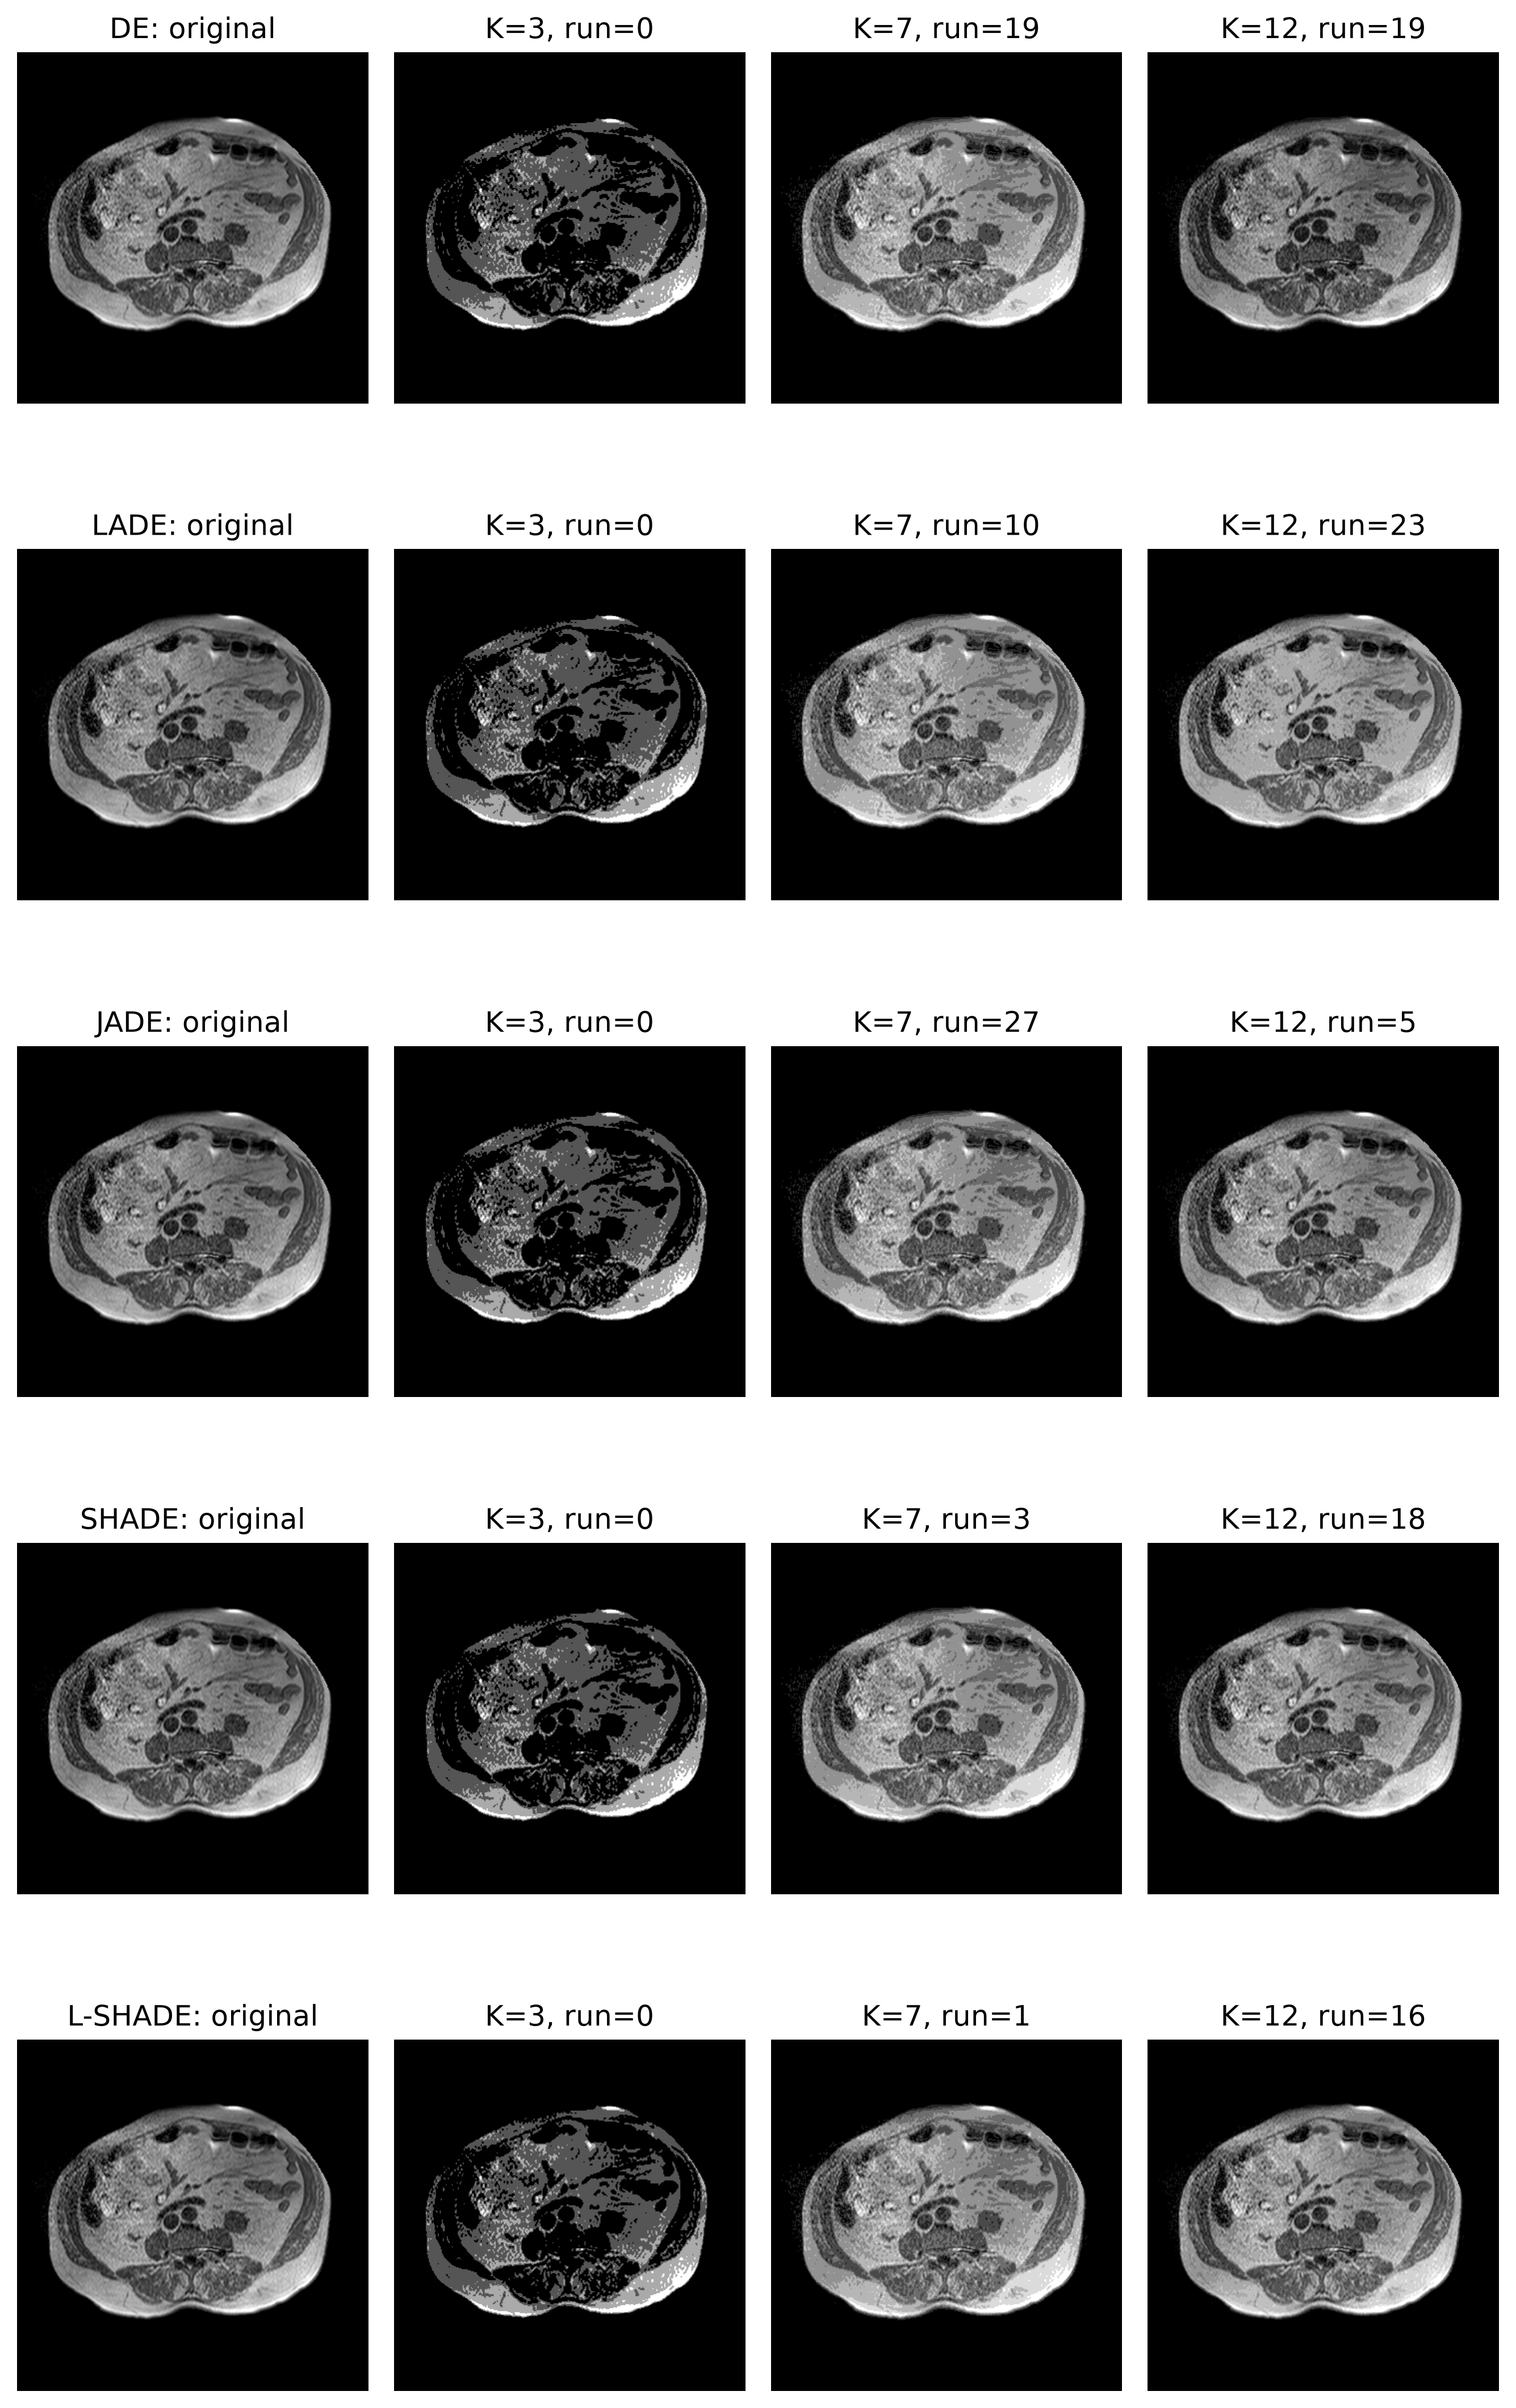
\includegraphics[width=0.9\textwidth]{exp2_segmentation_kapur.png}
\caption{Original and thresholded image IMG-0003-00010 using Kapur at $K=3,7,12$. Rows: DE, LADE, JADE, SHADE, L-SHADE. Solutions are selected by final fitness closest to the median, with ties resolved by the lowest run index. The displayed run number identifies an independent repetition.}
\label{fig:chaos-kapur}
\end{figure}

\begin{figure}[htbp]
\centering
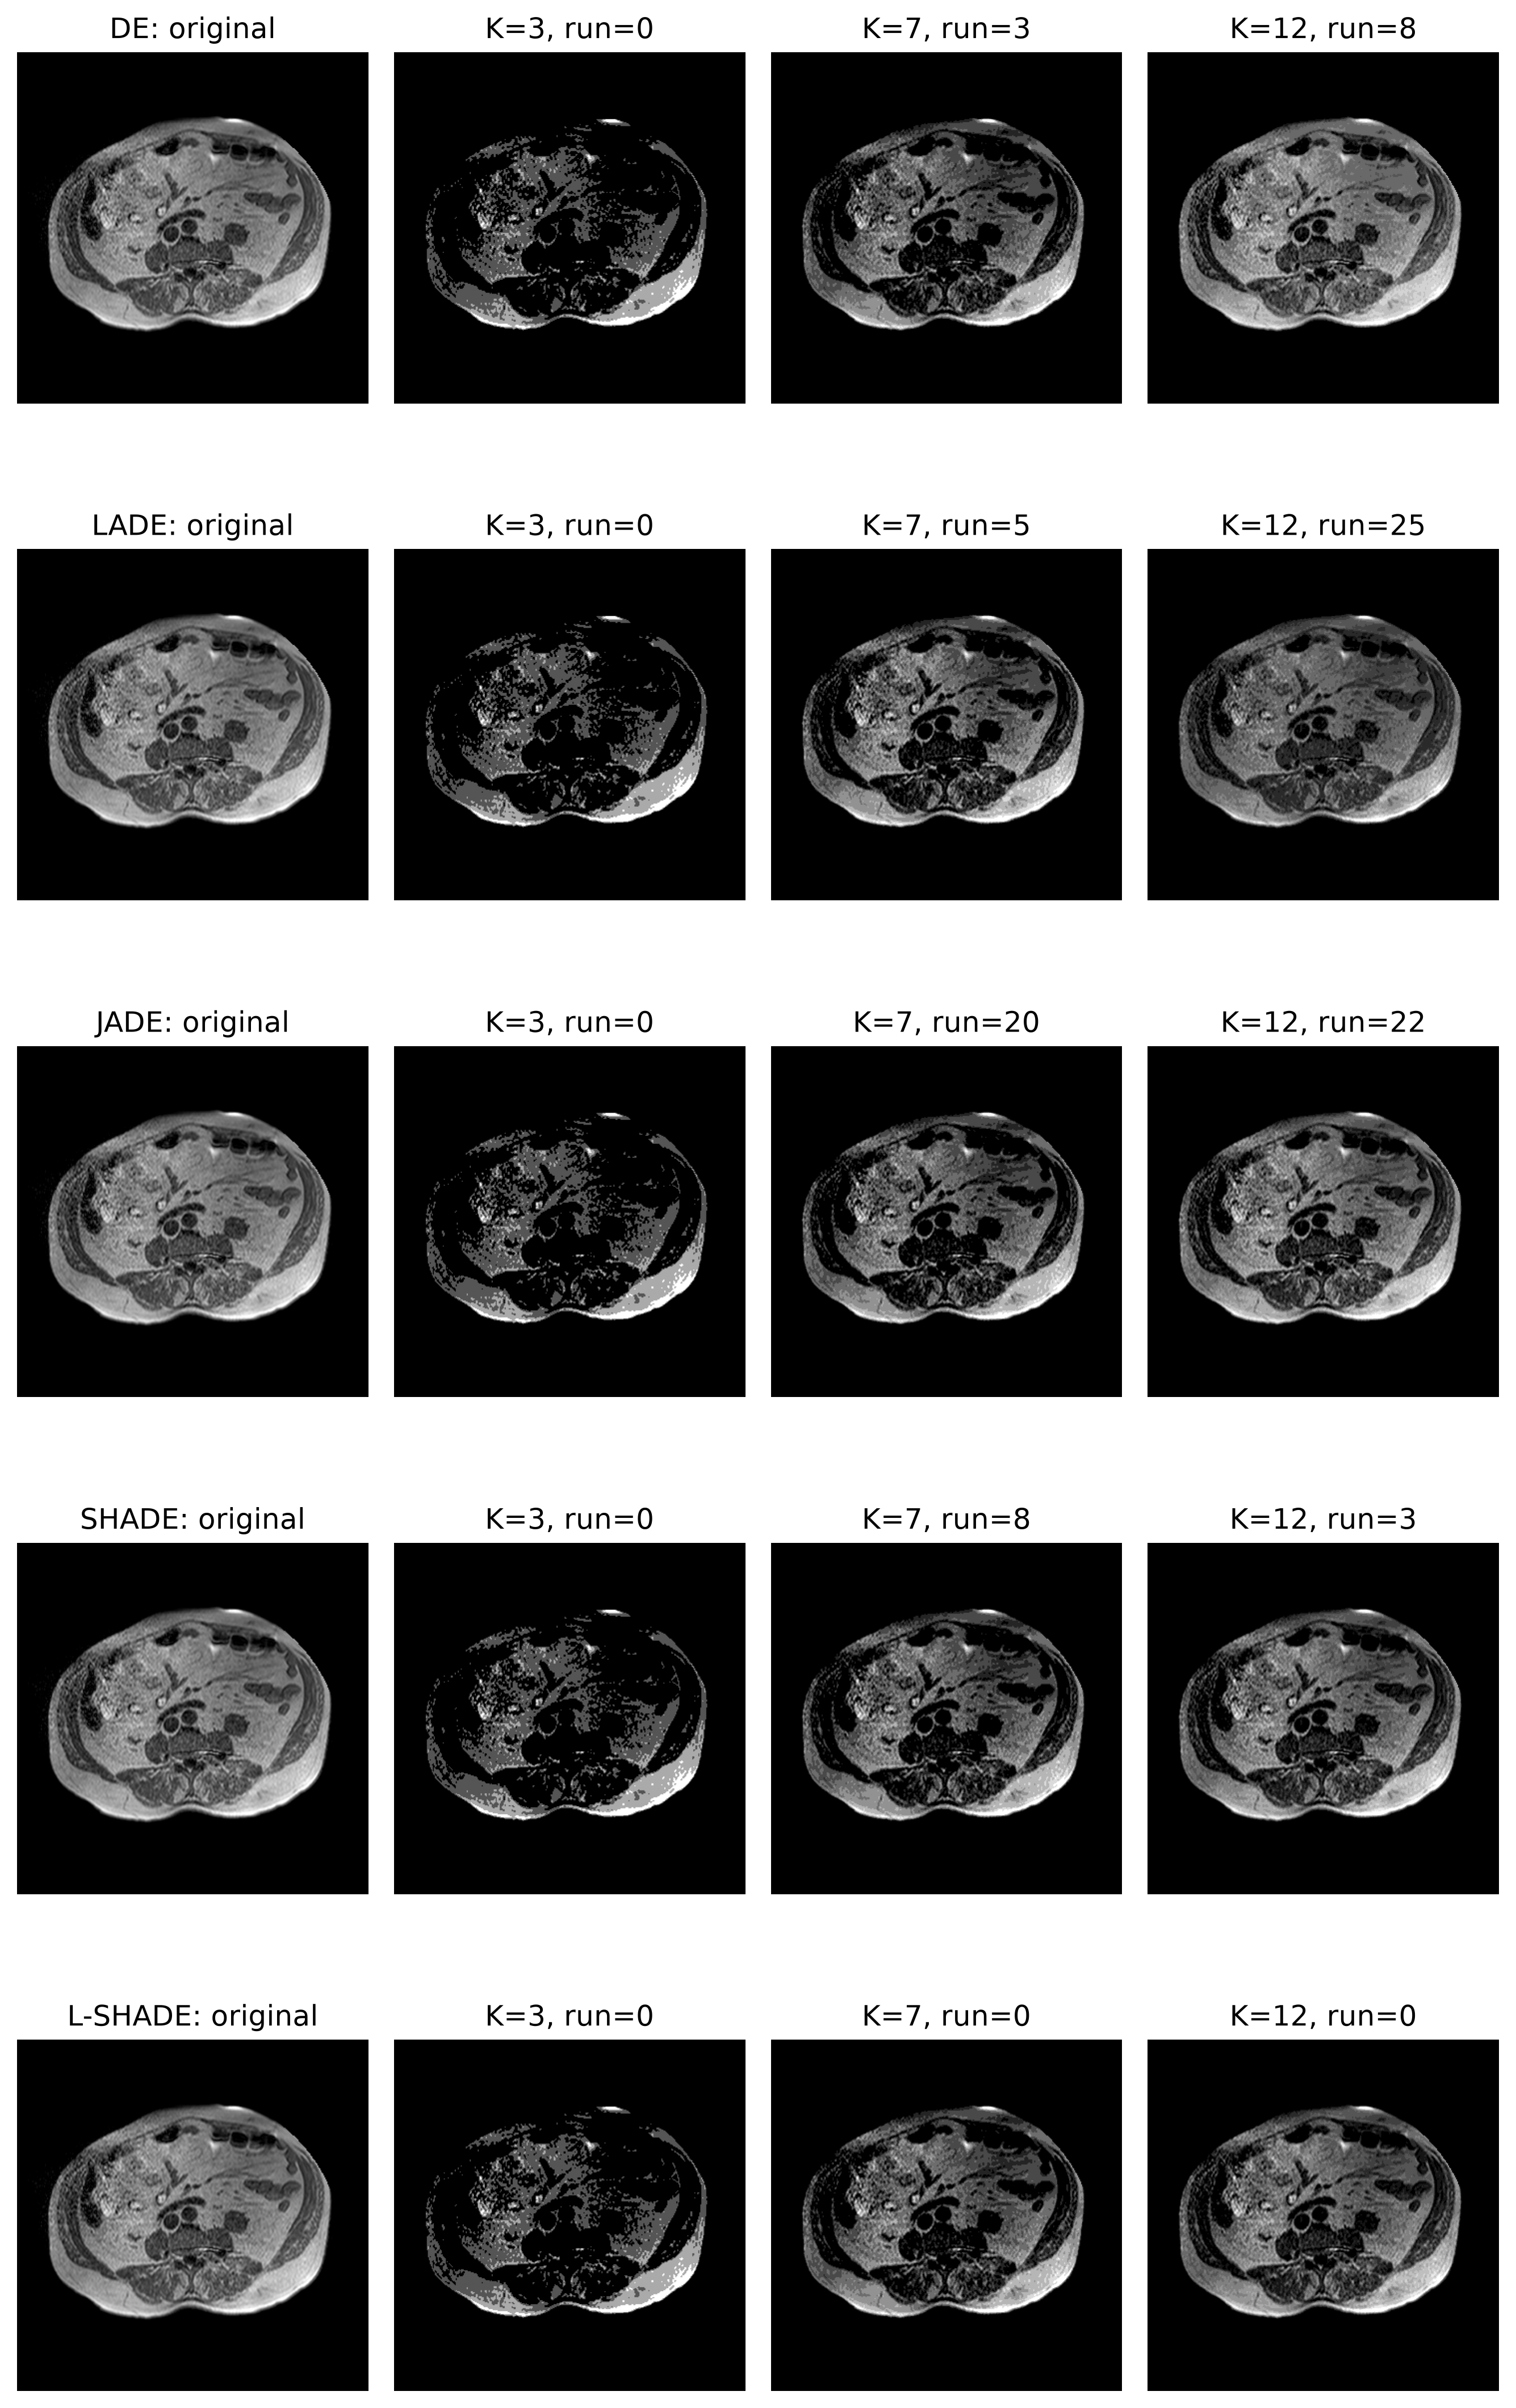
\includegraphics[width=0.9\textwidth]{exp2_segmentation_tsallis.png}
\caption{Original and thresholded image IMG-0003-00010 using Tsallis at $K=3,7,12$. Rows: DE, LADE, JADE, SHADE, L-SHADE. Solutions are selected by final fitness closest to the median, with ties resolved by the lowest run index. The displayed run number identifies an independent repetition.}
\label{fig:chaos-tsallis}
\end{figure}

\subsection{Convergence Analysis}

\begin{figure}[htbp]
\centering
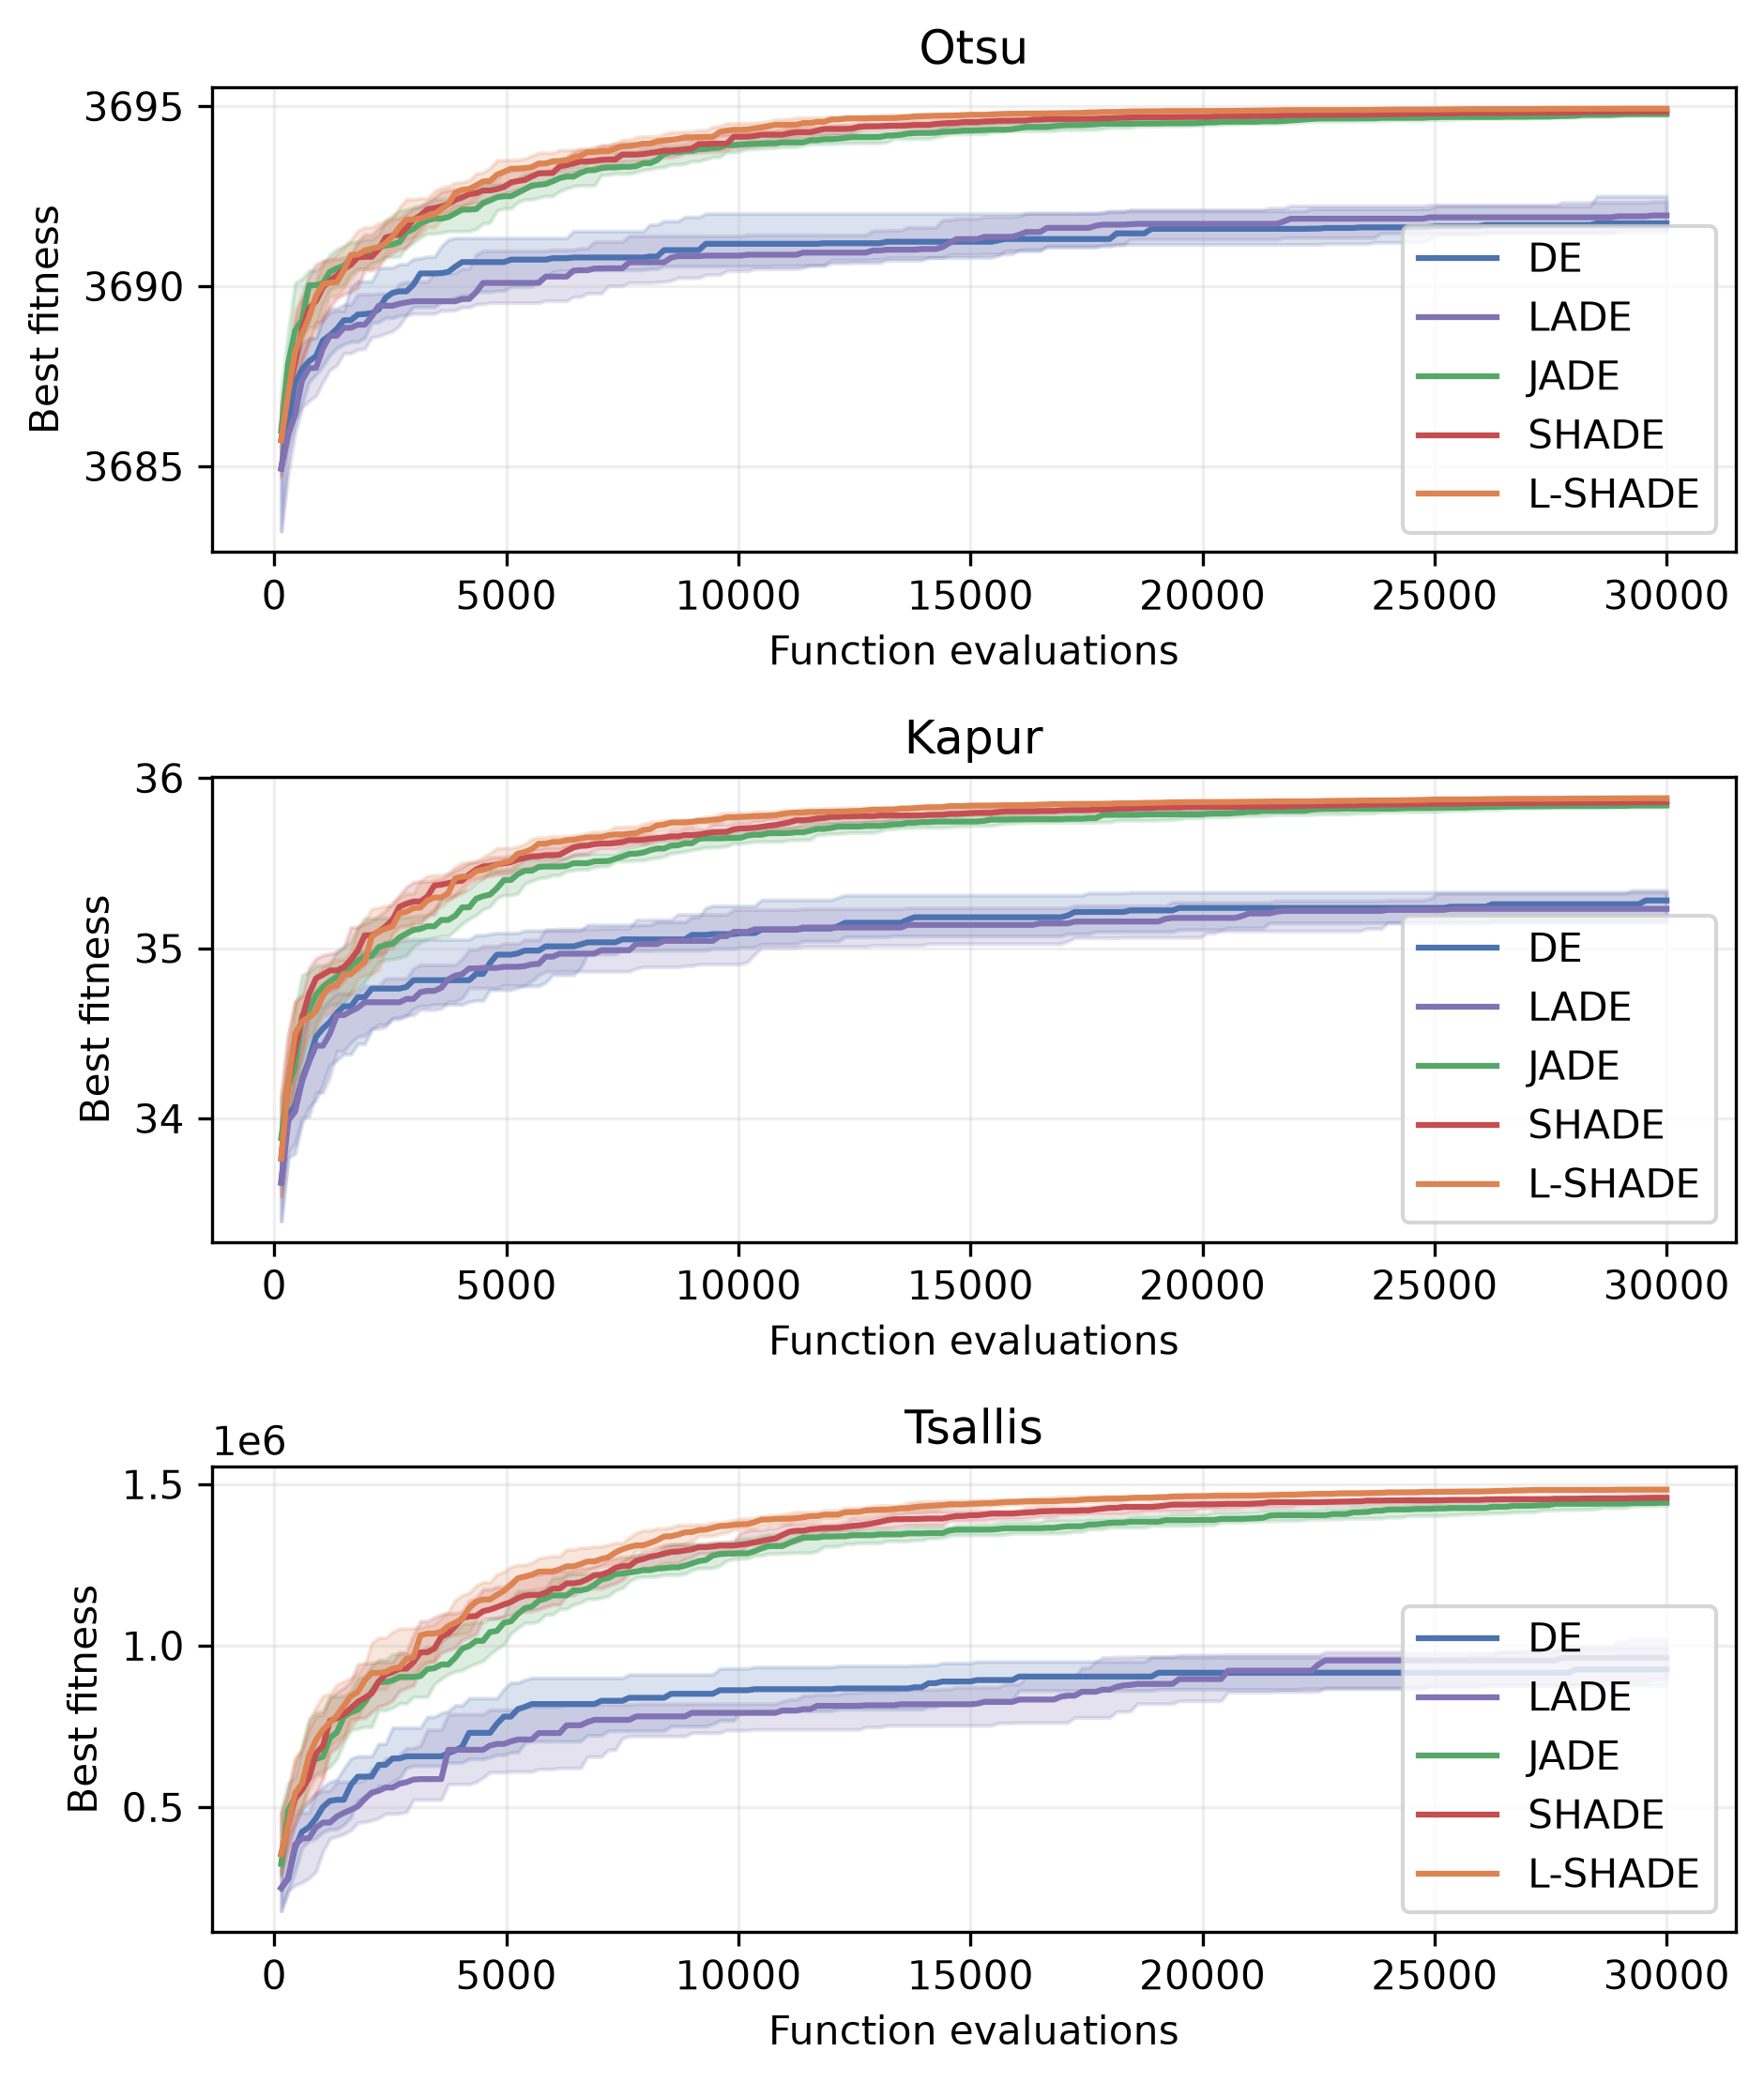
\includegraphics[width=0.9\textwidth]{exp2_convergence.png}
\caption{Best-so-far fitness for image IMG-0003-00010 at $K=12$. Lines show medians over 30 runs; bands show interquartile ranges.}
\label{fig:chaos-convergence}
\end{figure}

Figure~\ref{fig:chaos-convergence} shows nondecreasing best-so-far fitness
under the common evaluation budget. For this illustrative slice, the adaptive
SHADE variants continue improving later in the run, while gains generally
taper as the algorithms approach their final solutions.

\subsection{Execution Time}

\begin{figure}[htbp]
\centering
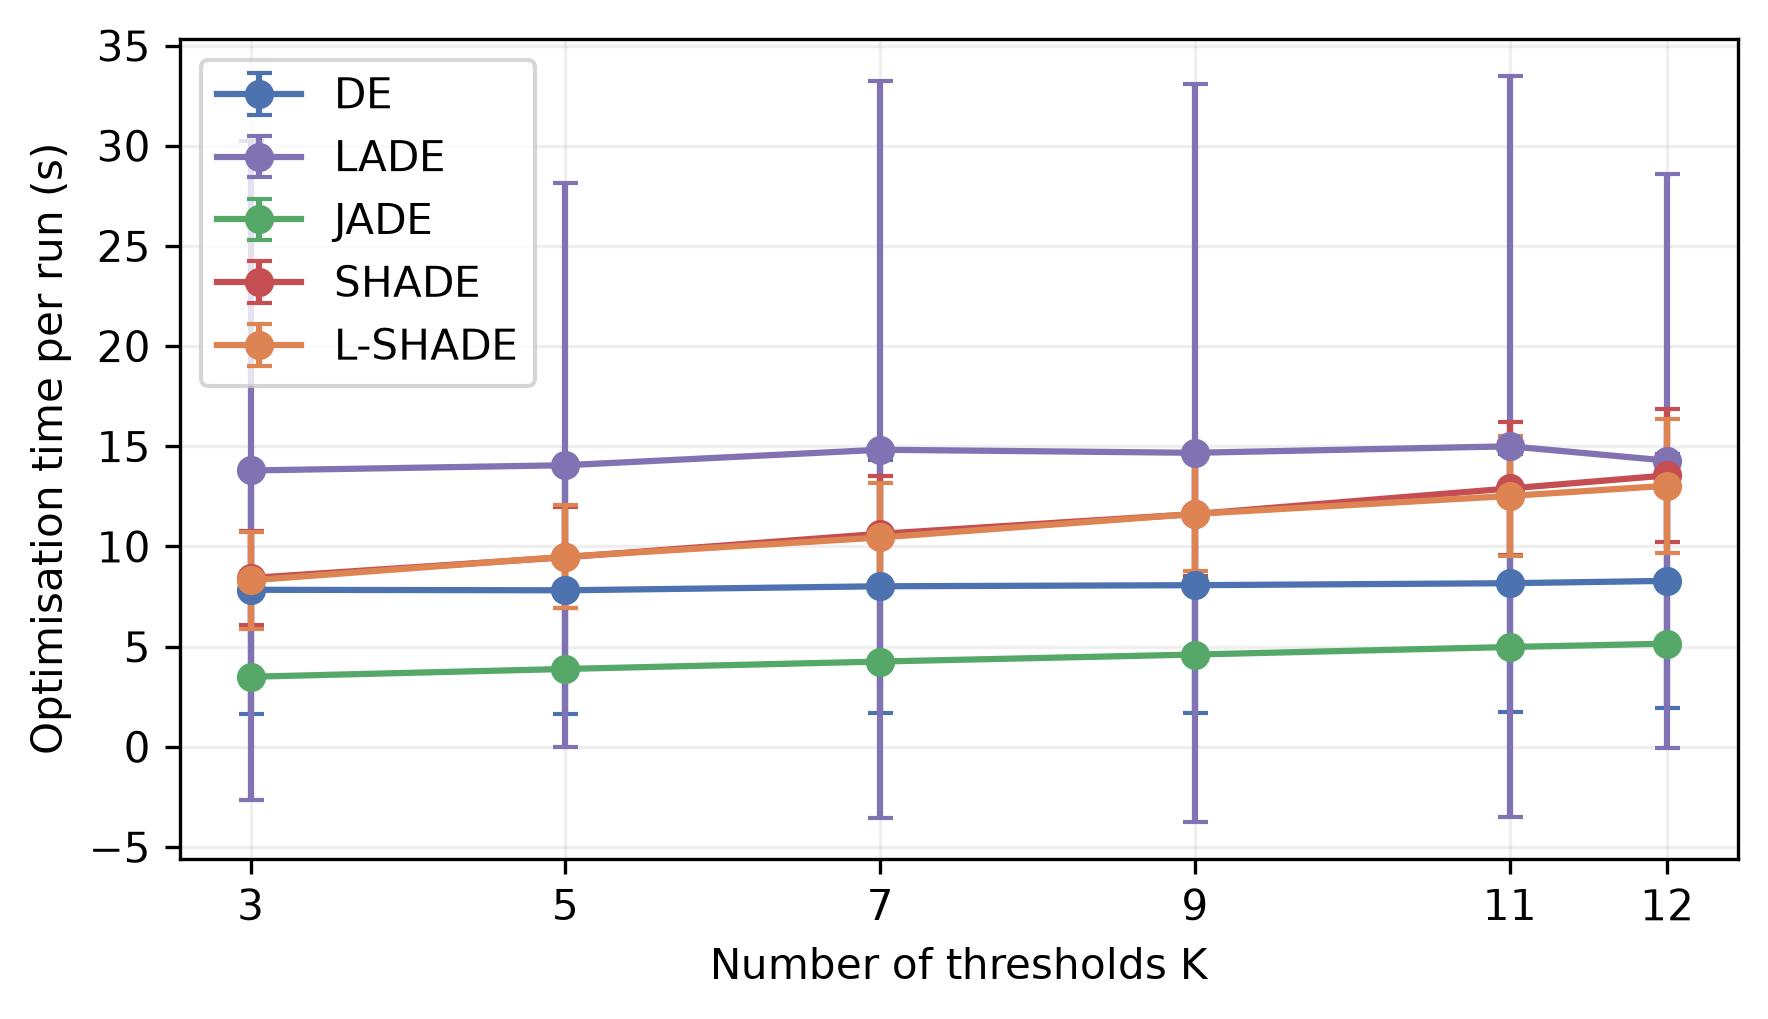
\includegraphics[width=0.9\textwidth]{exp2_runtime.png}
\caption{Mean recorded optimisation time versus $K$, with sample standard deviation as error bars, pooled across images, objectives and runs.}
\label{fig:chaos-runtime}
\end{figure}

Figure~\ref{fig:chaos-runtime} shows that the adaptive methods generally
become slower as $K$ increases, whereas DE and LADE are comparatively flat.
Because algorithms were executed in separate sessions, these timings are most
useful for assessing within-algorithm scaling rather than absolute speed.

\subsection{Discussion of Experiment 2}

Across the five algorithms, reconstruction quality generally improves as the
number of thresholds increases. The revised domain metric shows the same
strong dimensional trend. Averaged across algorithms, class separability for
Otsu rises from 0.975966 at $K=3$ to 0.997539 at $K=12$; Kapur rises from
0.910492 to 0.996838; and Tsallis rises from 0.812897 to 0.985168. Thus Otsu
separates the supplied MRI intensity classes most strongly at low $K$, while
the three objectives become closer as additional thresholds are introduced.

The best algorithmic values within a fixed objective and $K$ are much closer
than the differences caused by objective choice or threshold count. For
example, L-SHADE gives the highest mean Otsu separability from $K=5$ through
$K=12$, whereas the leader changes across $K$ for Kapur and Tsallis. These
small descriptive differences should be interpreted alongside the paired
fitness tests rather than as evidence of significance. Finally, a value near
one means that the threshold classes explain most of the image's intensity
variance; it does not establish that the classes correspond to anatomical
organs or clinically correct boundaries.

\section{Statistical Analysis}
\label{sec:statistics}

Because stochastic evolutionary algorithms may produce different
solutions across independent runs, statistical tests are used to
determine whether observed performance differences are statistically
significant.

A significance level of

\begin{equation}
\alpha = 0.05
\end{equation}

is used.


\subsection{Wilcoxon Signed-Rank Test}

Within each dataset--objective--$K$ cell, the pairwise analysis
uses the median fitness over 30 runs for each image. Algorithm values are
therefore paired by image, and the two-sided Wilcoxon signed-rank test
tests the null hypothesis that the paired differences are centred at
zero. Holm correction controls the family-wise error rate across the
algorithm pairs within a cell. Rank-biserial correlation is reported as
an effect size, with its sign oriented so that a positive value favours
the first algorithm. Of the 360 corrected pairwise comparisons (two
datasets, three objectives, six values of $K$ and ten algorithm pairs),
221 are significant. Table~\ref{tab:wilcoxon-summary} aggregates the 36
dataset--objective--$K$ cells for each pair; ``ties'' denote cells that
are not significant after Holm correction rather than identical scores.

\begin{table}[htbp]
\caption{Holm-corrected Wilcoxon significant wins, non-significant ties
and significant losses over 36 dataset--objective--$K$ cells. Counts are
from the perspective of the first named algorithm.}
\label{tab:wilcoxon-summary}
\centering
\begin{tabular}{lrrr}
\toprule
Comparison & Wins & Ties & Losses \\
\midrule
DE vs JADE & 0 & 14 & 22 \\
DE vs SHADE & 0 & 14 & 22 \\
DE vs L-SHADE & 0 & 13 & 23 \\
DE vs LADE & 10 & 26 & 0 \\
JADE vs SHADE & 0 & 12 & 24 \\
JADE vs L-SHADE & 0 & 12 & 24 \\
JADE vs LADE & 24 & 12 & 0 \\
SHADE vs L-SHADE & 0 & 12 & 24 \\
SHADE vs LADE & 24 & 12 & 0 \\
L-SHADE vs LADE & 24 & 12 & 0 \\
\bottomrule
\end{tabular}
\end{table}


\subsection{Friedman Test}

The omnibus comparison treats each image--$K$ combination as a
block and the five algorithms as treatments, using the median over the
30 runs for each block. The Friedman null hypothesis is that the
algorithms have equivalent ranks. The Iman--Davenport correction is used
for the omnibus significance decision, followed by a Nemenyi critical
difference comparison of mean ranks. All planned blocks are complete:
60 for each BSD500 objective and 90 for each CHAOS objective. The null
hypothesis is rejected for every dataset--objective combination
(Table~\ref{tab:friedman-results}). L-SHADE has the lowest (best) mean
rank in all six comparisons, followed by SHADE and JADE.


\begin{table}[H]
\caption{Friedman tests with Iman--Davenport correction. Rank order is
from best (lowest mean rank) to worst.}
\label{tab:friedman-results}
\centering
\small
\resizebox{\textwidth}{!}{%
\begin{tabular}{llrrrl}
\toprule
Dataset & Objective & Blocks & $F_{ID}$ & $p_{ID}$ & Mean-rank order \\
\midrule
BSD500 & Otsu & 60 & 76.786 & $1.302\times10^{-41}$ & L-SHADE $<$ SHADE $<$ JADE $<$ DE $<$ LADE \\
BSD500 & Kapur & 60 & 108.551 & $2.513\times10^{-52}$ & L-SHADE $<$ SHADE $<$ JADE $<$ DE $<$ LADE \\
BSD500 & Tsallis & 60 & 100.074 & $1.117\times10^{-49}$ & L-SHADE $<$ SHADE $<$ JADE $<$ DE $<$ LADE \\
CHAOS & Otsu & 90 & 129.404 & $4.269\times10^{-68}$ & L-SHADE $<$ SHADE $<$ JADE $<$ DE $<$ LADE \\
CHAOS & Kapur & 90 & 145.262 & $1.703\times10^{-73}$ & L-SHADE $<$ SHADE $<$ JADE $<$ DE $<$ LADE \\
CHAOS & Tsallis & 90 & 156.346 & $4.669\times10^{-77}$ & L-SHADE $<$ SHADE $<$ JADE $<$ DE $<$ LADE \\
\bottomrule
\end{tabular}
}

\end{table}

The Nemenyi critical difference is 0.787 for BSD500 and 0.643 for
CHAOS. The complete per-cell Wilcoxon statistics, Holm-adjusted
$p$-values, rank-biserial effects, Friedman ranks and critical-difference
diagrams are retained with the generated analysis artifacts.

\begin{figure*}[htbp]
\centering
\begin{subfigure}{0.32\textwidth}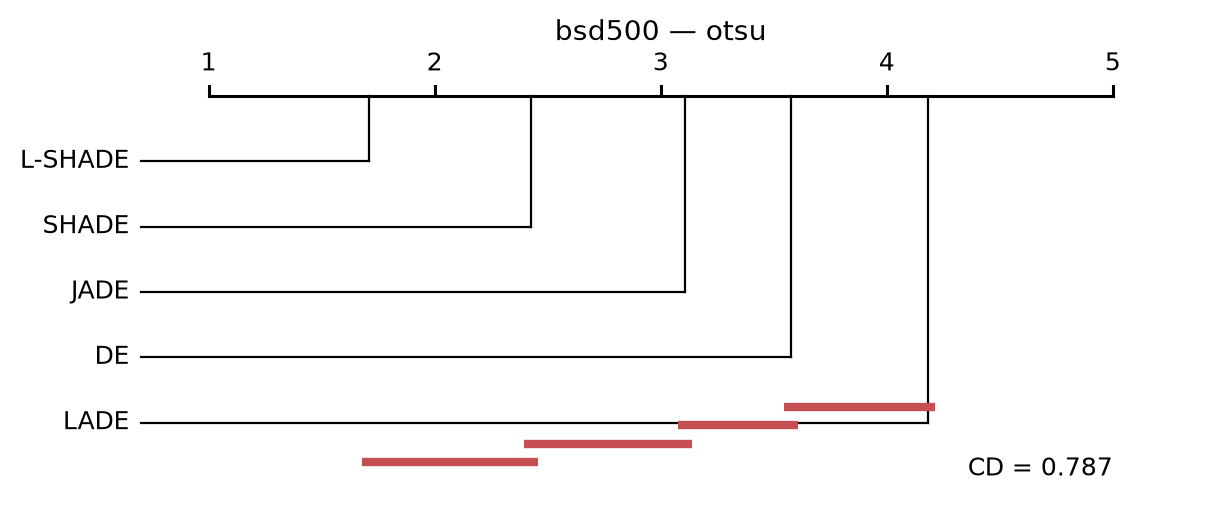
\includegraphics[width=\linewidth]{cd_bsd500_otsu.png}\caption{Otsu}\end{subfigure}
\begin{subfigure}{0.32\textwidth}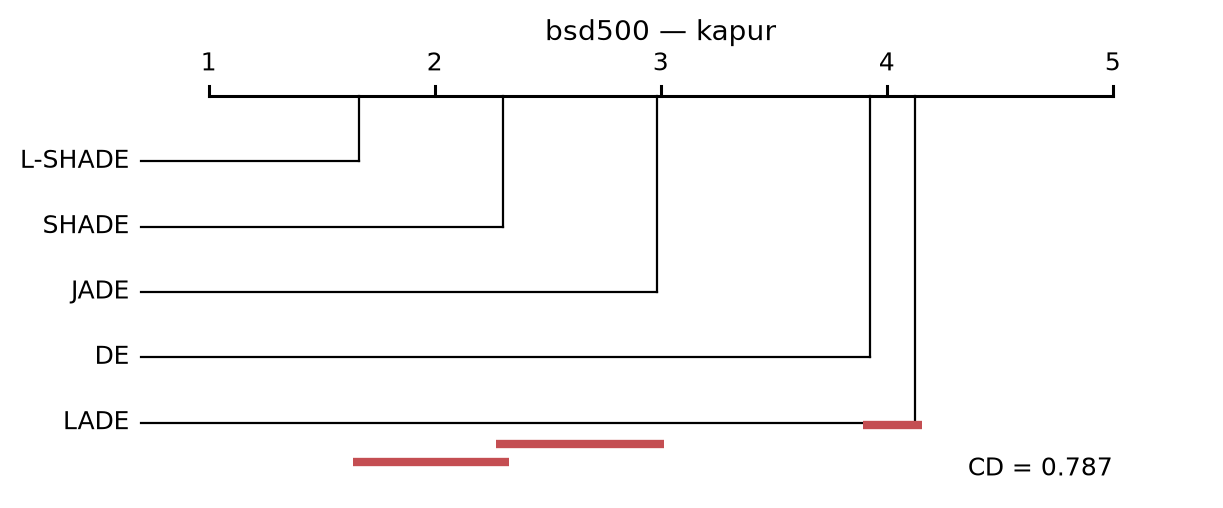
\includegraphics[width=\linewidth]{cd_bsd500_kapur.png}\caption{Kapur}\end{subfigure}
\begin{subfigure}{0.32\textwidth}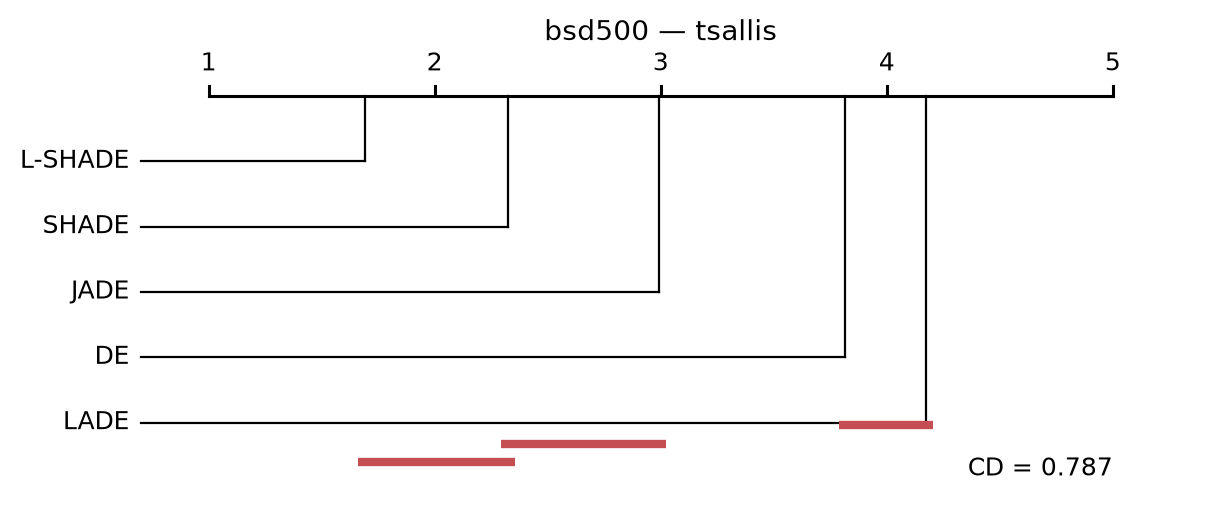
\includegraphics[width=\linewidth]{cd_bsd500_tsallis.png}\caption{Tsallis}\end{subfigure}
\caption{Nemenyi critical-difference diagrams for BSD500. Algorithms joined
by a horizontal bar are not separated by more than the critical difference.}
\label{fig:cd-bsd500}
\end{figure*}

\begin{figure*}[htbp]
\centering
\begin{subfigure}{0.32\textwidth}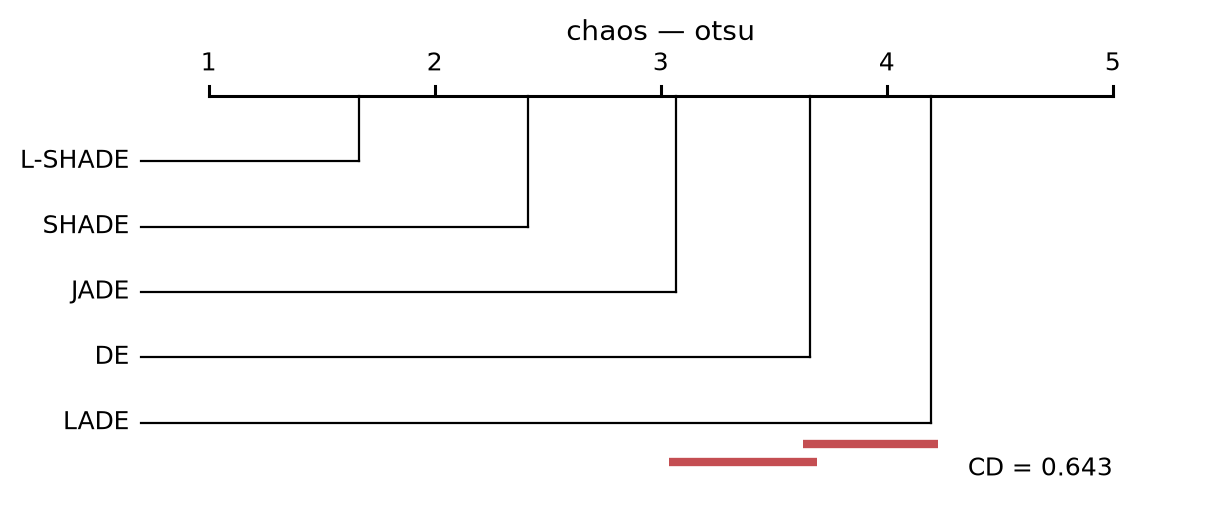
\includegraphics[width=\linewidth]{cd_chaos_otsu.png}\caption{Otsu}\end{subfigure}
\begin{subfigure}{0.32\textwidth}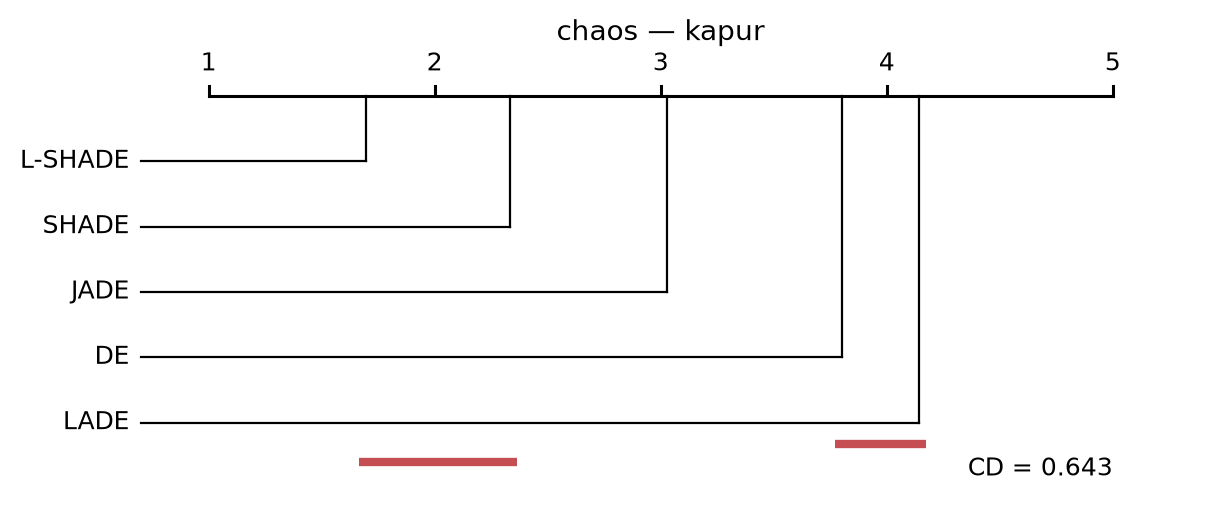
\includegraphics[width=\linewidth]{cd_chaos_kapur.png}\caption{Kapur}\end{subfigure}
\begin{subfigure}{0.32\textwidth}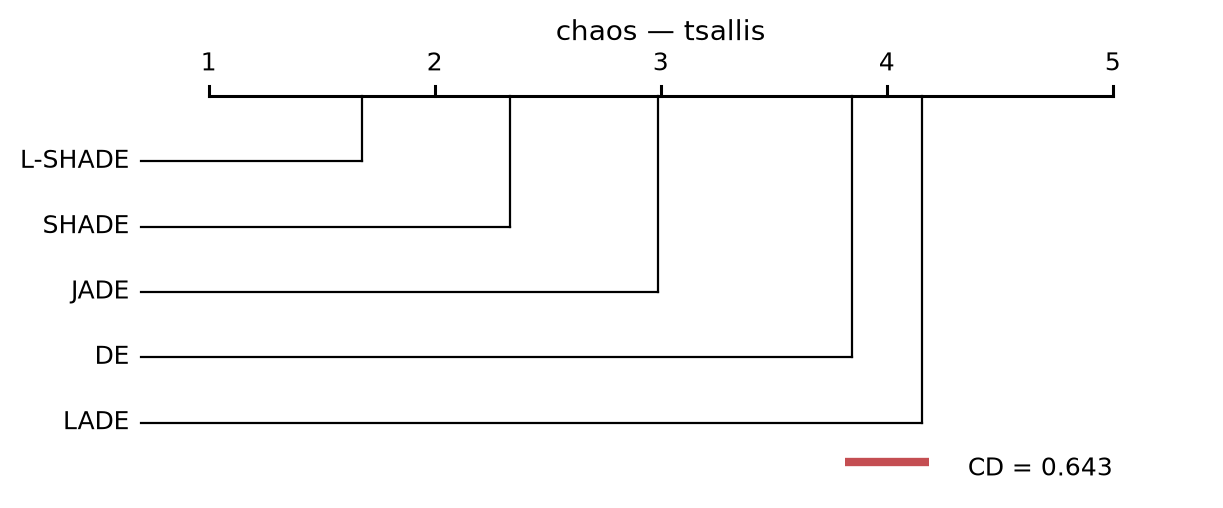
\includegraphics[width=\linewidth]{cd_chaos_tsallis.png}\caption{Tsallis}\end{subfigure}
\caption{Nemenyi critical-difference diagrams for CHAOS MRI. Lower mean rank
is better; connecting bars denote groups not separated by the critical
difference.}
\label{fig:cd-chaos}
\end{figure*}



% 9. SCALABILITY AND COMPUTATIONAL ANALYSIS


\section{Computational Scalability Analysis}
\label{sec:scalability}


\subsection{Execution Time versus Number of Thresholds}

\begin{figure*}[htbp]
\centering
\begin{subfigure}{0.49\textwidth}
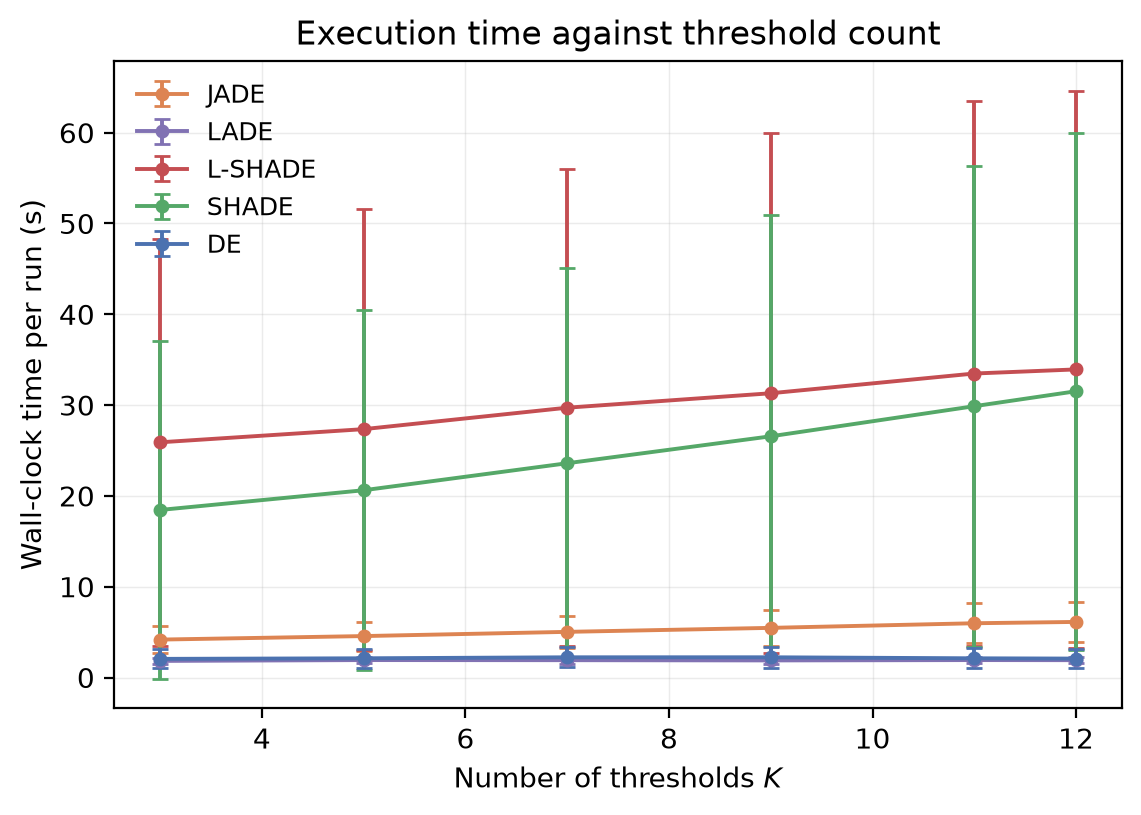
\includegraphics[width=\linewidth]{scalability_time_vs_k_bsd500.png}
\caption{BSD500}
\end{subfigure}
\begin{subfigure}{0.49\textwidth}
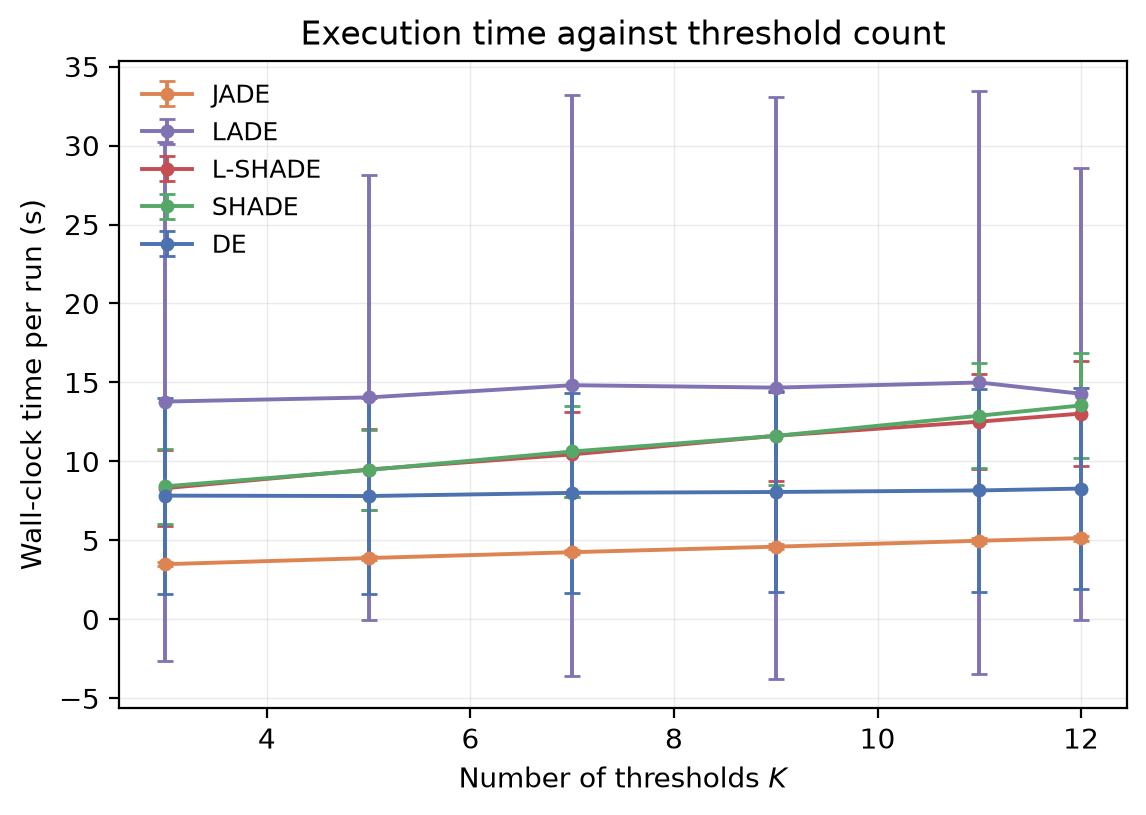
\includegraphics[width=\linewidth]{scalability_time_vs_k_chaos.png}
\caption{CHAOS MRI}
\end{subfigure}
\caption{Mean optimiser wall time for 30,000 objective evaluations as $K$
increases. Error bars show one standard deviation over objectives, images and
runs.}
\label{fig:runtime}
\end{figure*}

The timer surrounds only the optimiser call; image loading and post-run PSNR,
SSIM, uniformity and separability calculations are excluded. Consequently,
Figure~\ref{fig:runtime} compares search overhead under the common 30,000-FE
budget. JADE rises from 4.18 to 6.12 seconds on BSD500 and from 3.50 to
5.15 seconds on CHAOS as $K$ increases from 3 to 12. SHADE and L-SHADE show
larger increases: on CHAOS they rise from 8.42 to 13.55 seconds and from
8.31 to 13.03 seconds, respectively. Fixed-parameter DE and LADE are much
flatter with $K$, although absolute CHAOS timings differ from BSD500.

The extra cost of JADE, SHADE and L-SHADE is consistent with parameter
sampling, ranking and archive maintenance. Population reduction does not make
L-SHADE uniformly faster than SHADE: it reduces later population work, but
both implementations still consume exactly 30,000 objective evaluations and
their per-evaluation bookkeeping differs. Timings were collected during
separate experiment sessions and exhibit large standard deviations for some
algorithm--dataset groups; they support within-series scaling trends, not
hardware-independent speed rankings.


\subsection{Convergence Rate}

Figures~\ref{fig:bsd_convergence} and \ref{fig:chaos-convergence} plot median
best-so-far fitness against consumed function evaluations, with interquartile
ranges, for the common $K=12$ setting. Expressing the horizontal axis in FEs
rather than generations is important because L-SHADE changes population size.
The adaptive methods continue improving later in the budget and finish above
the fixed-parameter baselines in these illustrative cases, consistent with
the dataset-wide Friedman ranks. The curves are nevertheless for one image
per dataset; they illustrate search dynamics and are not used as an additional
significance test.


\subsection{Impact of Increasing Dimensionality}

The decision-vector dimension equals the number of thresholds, so the study
moves from a three-dimensional problem at $K=3$ to a 12-dimensional problem
at $K=12$. Even with ordering constraints, the number of feasible integer
threshold sets is $\binom{254}{K}$; hence the search space grows rapidly while
the FE budget remains fixed. Each objective evaluation also processes more
class intervals, explaining part of the timing increase.

Higher dimension therefore gives every method fewer effective opportunities
to explore each coordinate interaction. Fixed $F$ and $CR$ can lose diversity
or converge prematurely, while JADE and SHADE continually adapt these controls
and use archives to introduce displaced solutions. L-SHADE adds an explicit
exploration--exploitation schedule: a larger initial population samples the
expanded space, after which linear reduction concentrates the remaining
budget. Its best mean rank across all six dataset--objective analyses suggests
that this schedule remained effective over the tested dimensions, though the
experiment does not establish behaviour beyond $K=12$.



% 10. DISCUSSION


\section{Discussion}
\label{sec:discussion}



\subsection{Comparison of Differential Evolution Variants}

The variants differ chiefly in how they balance exploitation and
population diversity. DE uses fixed $F$ and $CR$ and provides the
baseline. JADE adapts these parameters using successful trials, employs
current-to-$p$best mutation and retains displaced solutions in an
archive. SHADE extends success-based adaptation with historical memories,
whereas L-SHADE additionally reduces its population as the evaluation
budget is consumed. LADE retains the fixed DE mutation and crossover
parameters but relaxes selection using historical fitness benchmarks.
The results show that no mechanism should be judged from a single
objective or $K$ value. Nevertheless, the fitness-rank analysis gives a
consistent ordering across objectives and datasets: L-SHADE ranks first,
followed by SHADE and JADE, while DE and LADE occupy the lower ranks.


\subsection{Impact of Objective Function}

Across both datasets, Otsu generally provides the strongest PSNR, SSIM
and uniformity, with Kapur usually close behind. Tsallis at $q=0.8$
often produces lower reconstruction scores, particularly at small and
moderate $K$. This does not imply that its entropy objective is being
optimised incorrectly: entropy maximisation and class-mean reconstruction
quality measure different properties of a threshold set.


\subsection{Impact of Tsallis Non-Extensivity Parameter}

The entropic index $q$ controls the non-additive weighting in Tsallis
entropy. This study fixes $q=0.8$ for every run, ensuring a fair
algorithm comparison but preventing conclusions about sensitivity to
$q$. The weaker reconstruction metrics observed for this configuration
may reflect the selected entropy criterion rather than the optimiser;
testing several $q$ values would be required to separate these effects.


\subsection{BSD500 versus CHAOS MRI}

BSD500 provides varied natural-image intensity distributions, while the
CHAOS subset contains grayscale abdominal MRI slices with different
contrast and tissue-intensity structure. Reconstruction metrics quantify
how well the class-mean image preserves the source, whereas the revised
CHAOS evaluation uses $\eta$ to quantify unsupervised intensity-class
separation. The latter is a domain-relevant partition-quality measure, but
it should not be interpreted as anatomical organ-recognition accuracy.


\subsection{Algorithm Robustness}

Robustness is assessed through 30 independent runs, pooled and per-image
standard deviations, and median convergence curves with interquartile
ranges. Pooled deviations also contain genuine between-image variation
and therefore should not be interpreted solely as stochastic algorithm
instability. Formal robustness comparisons remain conditional on the
completed paired statistical analysis.


\subsection{Limitations}

Possible limitations include:

\begin{itemize}
    \item evaluation on a limited number of images;
    \item dependence on selected DE parameter settings;
    \item use of only the fixed Tsallis value $q=0.8$;
    \item stochastic variability between runs;
    \item computational cost associated with repeated optimisation; and
    \item limitations of intensity-only thresholding for complex
          anatomical structures.
\end{itemize}



% 11. CONCLUSION


\section{Conclusion}
\label{sec:conclusion}

This study evaluated five Differential Evolution algorithms for
multilevel image thresholding using Otsu, Kapur, and Tsallis objective
functions across six threshold dimensions.
Across both datasets, reconstruction quality generally improves as more
thresholds are introduced, while objective choice materially affects
the resulting metrics. On CHAOS at $K=12$, L-SHADE gives the highest
mean Otsu PSNR, SHADE the highest mean Kapur PSNR, and LADE the highest
mean Tsallis PSNR. The omnibus tests reject equivalent fitness ranks in
all six dataset--objective comparisons, and L-SHADE has the best mean
fitness rank throughout. These fitness results should not be conflated
with reconstruction metrics, whose leading algorithm depends on the
selected objective.
For the revised CHAOS criterion, mean class separability increases with $K$
for all three objectives and reaches 0.997539 for Otsu, 0.996838 for Kapur and
0.985168 for Tsallis at $K=12$ when averaged across algorithms. Otsu is
strongest at low threshold counts, and objective differences narrow as $K$
increases. These values measure unsupervised intensity separation rather than
anatomical recognition accuracy.


% AUTHOR CONTRIBUTIONS


\section*{CRediT authorship contribution statement}

\textbf{Aryan Mohanlall:}
Standard DE and Late Acceptance DE implementation.

\textbf{Jaden Moodley:}

\textbf{Third Author:}

\textbf{Fourth Author:}`'



% DECLARATIONS


\section*{Declaration of Competing Interest}

The authors declare that they have no known competing financial
interests or personal relationships that could have appeared to
influence the work reported in this paper.


\section*{Acknowledgements}



\section*{Data availability}

The source code, experimental configurations, and generated results
used in this study are provided in the accompanying assignment
submission repository.




% REFERENCES


\bibliography{references}

\end{document}
